\documentclass[10pt,letterpaper]{article}
\usepackage{geometry}
\geometry{margin=1in}
\usepackage{graphicx}
\usepackage[dvipsnames]{xcolor}

\setlength{\parindent}{0pt}
\setlength{\parskip}{0.5em}

%make lists tighter
\usepackage{enumitem}
\setlist{nolistsep}

%reduce spacing before and after section
\usepackage{titlesec}
% reduce section, subsection, etc spacing
\usepackage{titlesec}
\titlespacing*{\section}{0pt}{0\baselineskip}{0\baselineskip}
\titlespacing*{\subsection}{0pt}{0\baselineskip}{0\baselineskip}
\titlespacing*{\subsubsection}{0pt}{0\baselineskip}{0\baselineskip}

%reduce list spacing
\usepackage{enumitem}
\setlist{nosep}

\usepackage[hidelinks]{hyperref}
\usepackage{biblatex}
\usepackage{subcaption}
\usepackage{multirow}
\usepackage{fix-cm}
\addbibresource{citations.bib}

\title{Lab 2 - Cloud Data, Stat 214, Spring 2025}

% submission must not contain any of your names
% but feel free to make a version for yourself with your names on it
\author{Anonymous}

\begin{document}
\maketitle

\section{Introduction}
% Why is the task important?
% Introduce the dataset
% Summarize what we are going to do in this lab

To better understand the relationship between increasing atmospheric carbon dioxide levels and global surface air temperatures, climate scientists require accurate measurements of cloud coverage. This is especially critical in the Arctic, where the distribution and scattering properties of snow, ice, atmospheric water vapor, and clouds have significant potential to change as temperatures rise. In these regions, surface albedo—the amount of solar radiation reflected to space by Earth's surface—is highly sensitive to increasing atmospheric carbon, creating a positive feedback loop. Therefore, accurate Arctic-wide measurements of cloud coverage are essential to understanding clouds' role in regulating the Arctic's sensitivity to global climate change.

Cloud detection, however, poses a major challenge in the Arctic because the infrared electromagnetic radiation emitted from clouds is similar to that of ice- and snow-covered surfaces. The launch of NASA's Terra satellite in 1999 provided a breakthrough with the Multiangle Imaging SpectroRadiometer (MISR), which captures electromagnetic radiation measurements at nine view zenith angles across four spectral bands. Despite this technological advancement, existing MISR operational algorithms remain ineffective at detecting clouds over bright surfaces in polar regions.

In this investigation, we will develop a cloud detection model trained on Arctic MISR data. We begin with an exploratory data analysis (EDA) of three expertly labeled MISR images, identifying patterns, relationships, and challenges in distinguishing cloud from non-cloud pixels. Insights from this analysis guide our feature engineering, where we transform the original MISR measurements into more discriminative representations to better separate clouds from the snow- and ice-covered surfaces that typically confound detection algorithms. Given the limited availability of labeled data, we employ an unsupervised representation learning approach: first, we train an autoencoder on a larger set of unlabeled MISR images to learn meaningful representations of Arctic scenes; then, we fine-tune it using our small labeled dataset. Finally, we evaluate and optimize the model's performance in identifying clouds, aiming to improve upon existing operational algorithms and contribute more accurate cloud detection capabilities for climate research in polar regions.

\subsection{Dataset}

The dataset from \cite{shi2008daytime} consists of $164$ MISR images, each with a resolution of approximately $304 \times 382$ pixels. For each pixel, the dataset includes $(x, y)$ coordinates, five angular radiances captured by different cameras (Df, Cf, Bf, Af, An), and three derived features:

\begin{itemize}
    \item \textbf{CORR}: The average linear correlation of radiation measurements across different viewing angles. High CORR values indicate either clear (cloud-free) conditions or the presence of low-altitude clouds that align with the surface below.
    \item \textbf{SD}: The standard deviation of red-band radiation measurements from the MISR An camera within small pixel groups. Low SD values suggest smooth surfaces where variations are primarily due to instrument noise.
    \item \textbf{NDAI}: A function of Df and An camera measurements designed to capture the contrast observed over Arctic clouds, where radiation from the Df camera is typically much higher than from the An camera. Larger NDAI values suggest cloud presence.
\end{itemize}

Additionally, three of the MISR images include expert-labeled annotations, where each pixel is categorized as cloud (+1), non-cloud (-1), or unlabeled (0).

\section{EDA}
% For the 3 labeled images, plot the expert labels for the presence or absence of clouds according to a map (i.e.~use the X, Y coordinates).

% Also plot the features (selected channels)

% Explore the relationships between the radiances of different angles, both visually and quantitatively. Do you notice differences between the two classes (cloud, no cloud) based on the radiances? Are there differences based on the features (CORR, NDAI, SD)?

% Describe our splitting strategy for the data (3 labeled images, 2 for training and validation (cross-validation), 1 for testing). Justify why we choose to use an image-level split instead of a pixel-level or patch-level split. (Reasons could include the fact that the algorithm will be applied to new images in the future, and we want to evaluate the algorithm's performance on new images. The patterns in different images could be different - position, brightness, proportion of clouded pixels, etc, so we want to make sure the algorithm can generalize to new images.)

% As is common when dealing with real-world data, these images may have imperfections that you'll need to clean up. Recall the skills you developed during Lab 1.

% (missing values at the edges. Claim that padding with 0 is a reasonable strategy for this dataset because the prediction is pixel-wise, and missing pixels are not counted in the loss function. Also, it's the default strategy in deep learning)

% (Noise. Claim that the noise is not too severe, and deep learning models are robust to noise. Also, the noise is not systematic, and trying to remove it might introduce bias.)

% (Outliers. Claim that no significant outliers are present in the data.)

In this section, we conduct an EDA of the MISR dataset to get a better understanding of the data and identify patterns that may inform our feature engineering and modeling strategies. We begin by visualizing the expert-labeled annotations for the three MISR images, highlighting the spatial distribution of cloud and non-cloud pixels. Next, we explore the relationships between the angular radiances and the derived features (CORR, SD, NDAI) to identify differences between cloud and non-cloud pixels. Finally, we describe our data-splitting strategy, justify the image-level split, and address potential data imperfections.

\subsection{Visualizations}

In Figure \ref{fig:map}, we visualize the expert-labeled annotations for each of the three MISR images. The cloud formations vary in size and shape—some are large and rounded, while others are thin and wispy. Additionally, the unlabeled pixels form a noticeable margin between cloud and non-cloud regions, with the width of this margin varying across images. Notably, no cloud-labeled and non-cloud-labeled pixels directly border each other at any point.

\begin{figure}[ht]
    \centering
    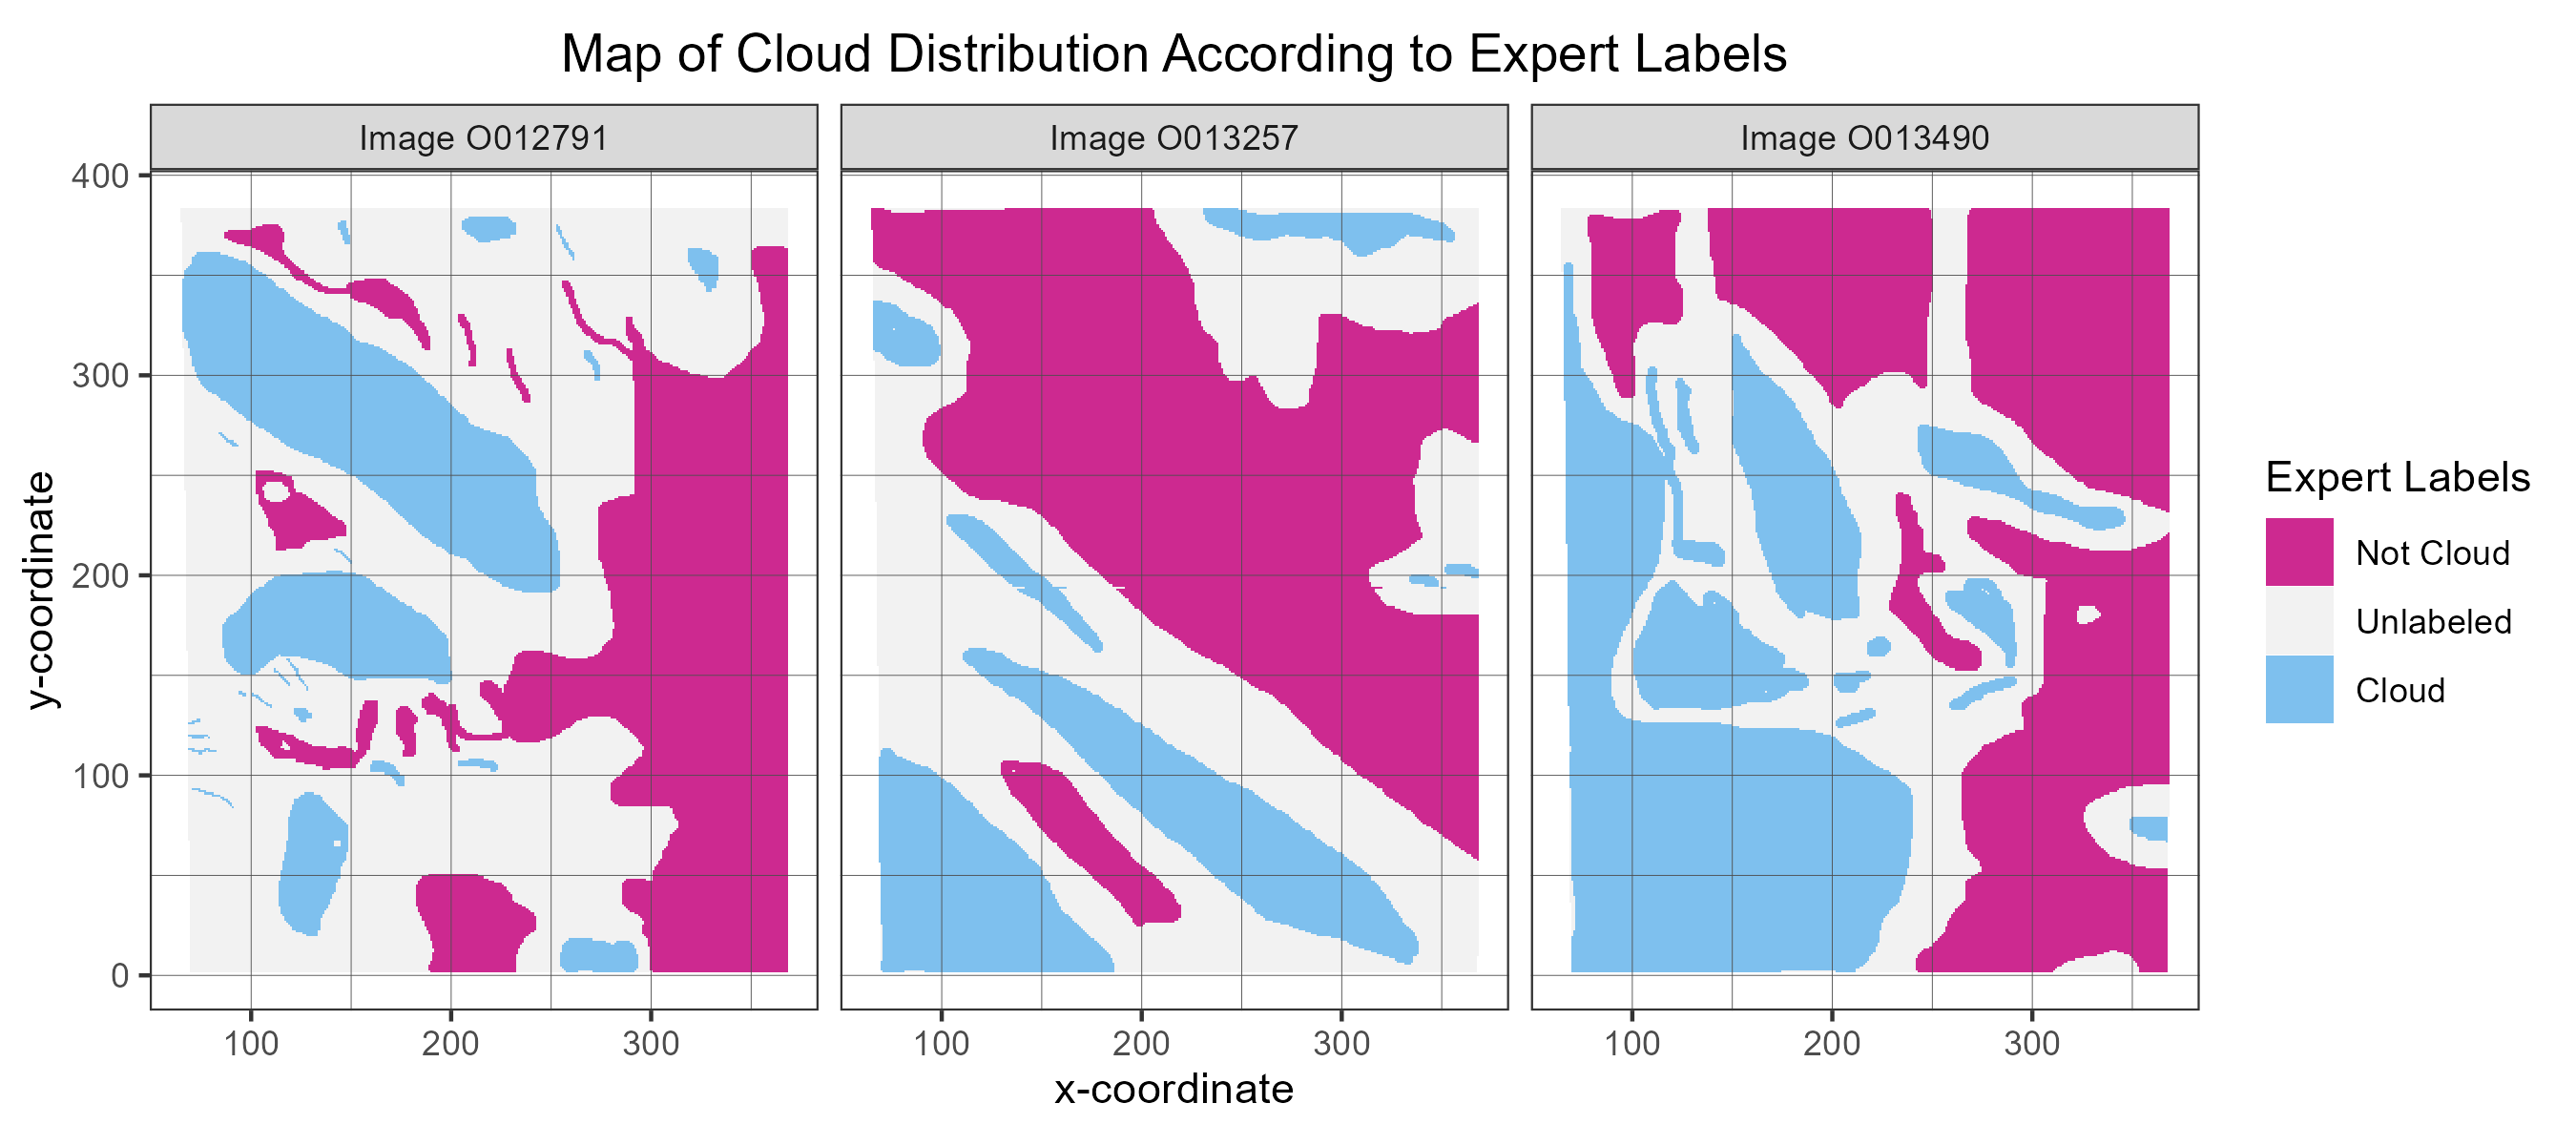
\includegraphics[width=\textwidth]{figs/map.png}
    \caption{Expert labels, mapped onto the three annotated MISR images, reveal substantial variation in cloud shape, size, and the boundaries between labeled regions.}
    \label{fig:map}
\end{figure}

In Figure \ref{fig:corr_combined},  we present scatterplot matrices of the five angular radiances for each annotated image. Since we are primarily interested in the "+1" (cloud) and "-1" (non-cloud) labels, and because the dataset is large and imbalanced, we plot only a balanced subsample of $n=10,000$ pixels. We observe strong positive linear relationships across nearly all pairs of radiance angles, with one notable exception: scatterplots involving the DF camera from image O013490. Pixels are color-coded light blue for clouds and maroon for non-clouds. In each image, non-cloud pixels form a distinct distribution that repeats across most radiance-angle pairs. This pattern aligns with the marginal densities (plotted along the diagonals), where non-cloud pixels exhibit a sharp, concentrated peak in radiance values, while cloud pixels are more widely distributed. This behavior is expected, as clouds are closer to the satellite than the ground surface, causing greater variation in angular radiances. Even with just these five features, cloud and non-cloud pixels already appear to be well-separated.

\begin{figure}[ht]
    \centering

    % Added title and subtitle to figure
    % and removed them from the subplots
    % corr{N}.png  vs. corr{N}_void.png
    \parbox{\textwidth}{\centering 
        \fontsize{13pt}{13pt}\selectfont \textbf{Scatterplot Matrix of Radiance Angles}  
        
        {\fontsize{11pt}{13pt}\selectfont Comparing equal subsamples of pixels labeled as \textcolor{Cyan}{\textbf{Cloud}} vs. \textcolor{RedViolet}{\textbf{Non-Cloud}}.} 
    }
    
    \begin{subfigure}[t]{0.3\textwidth}
        \centering
        \caption{Image O012791}
        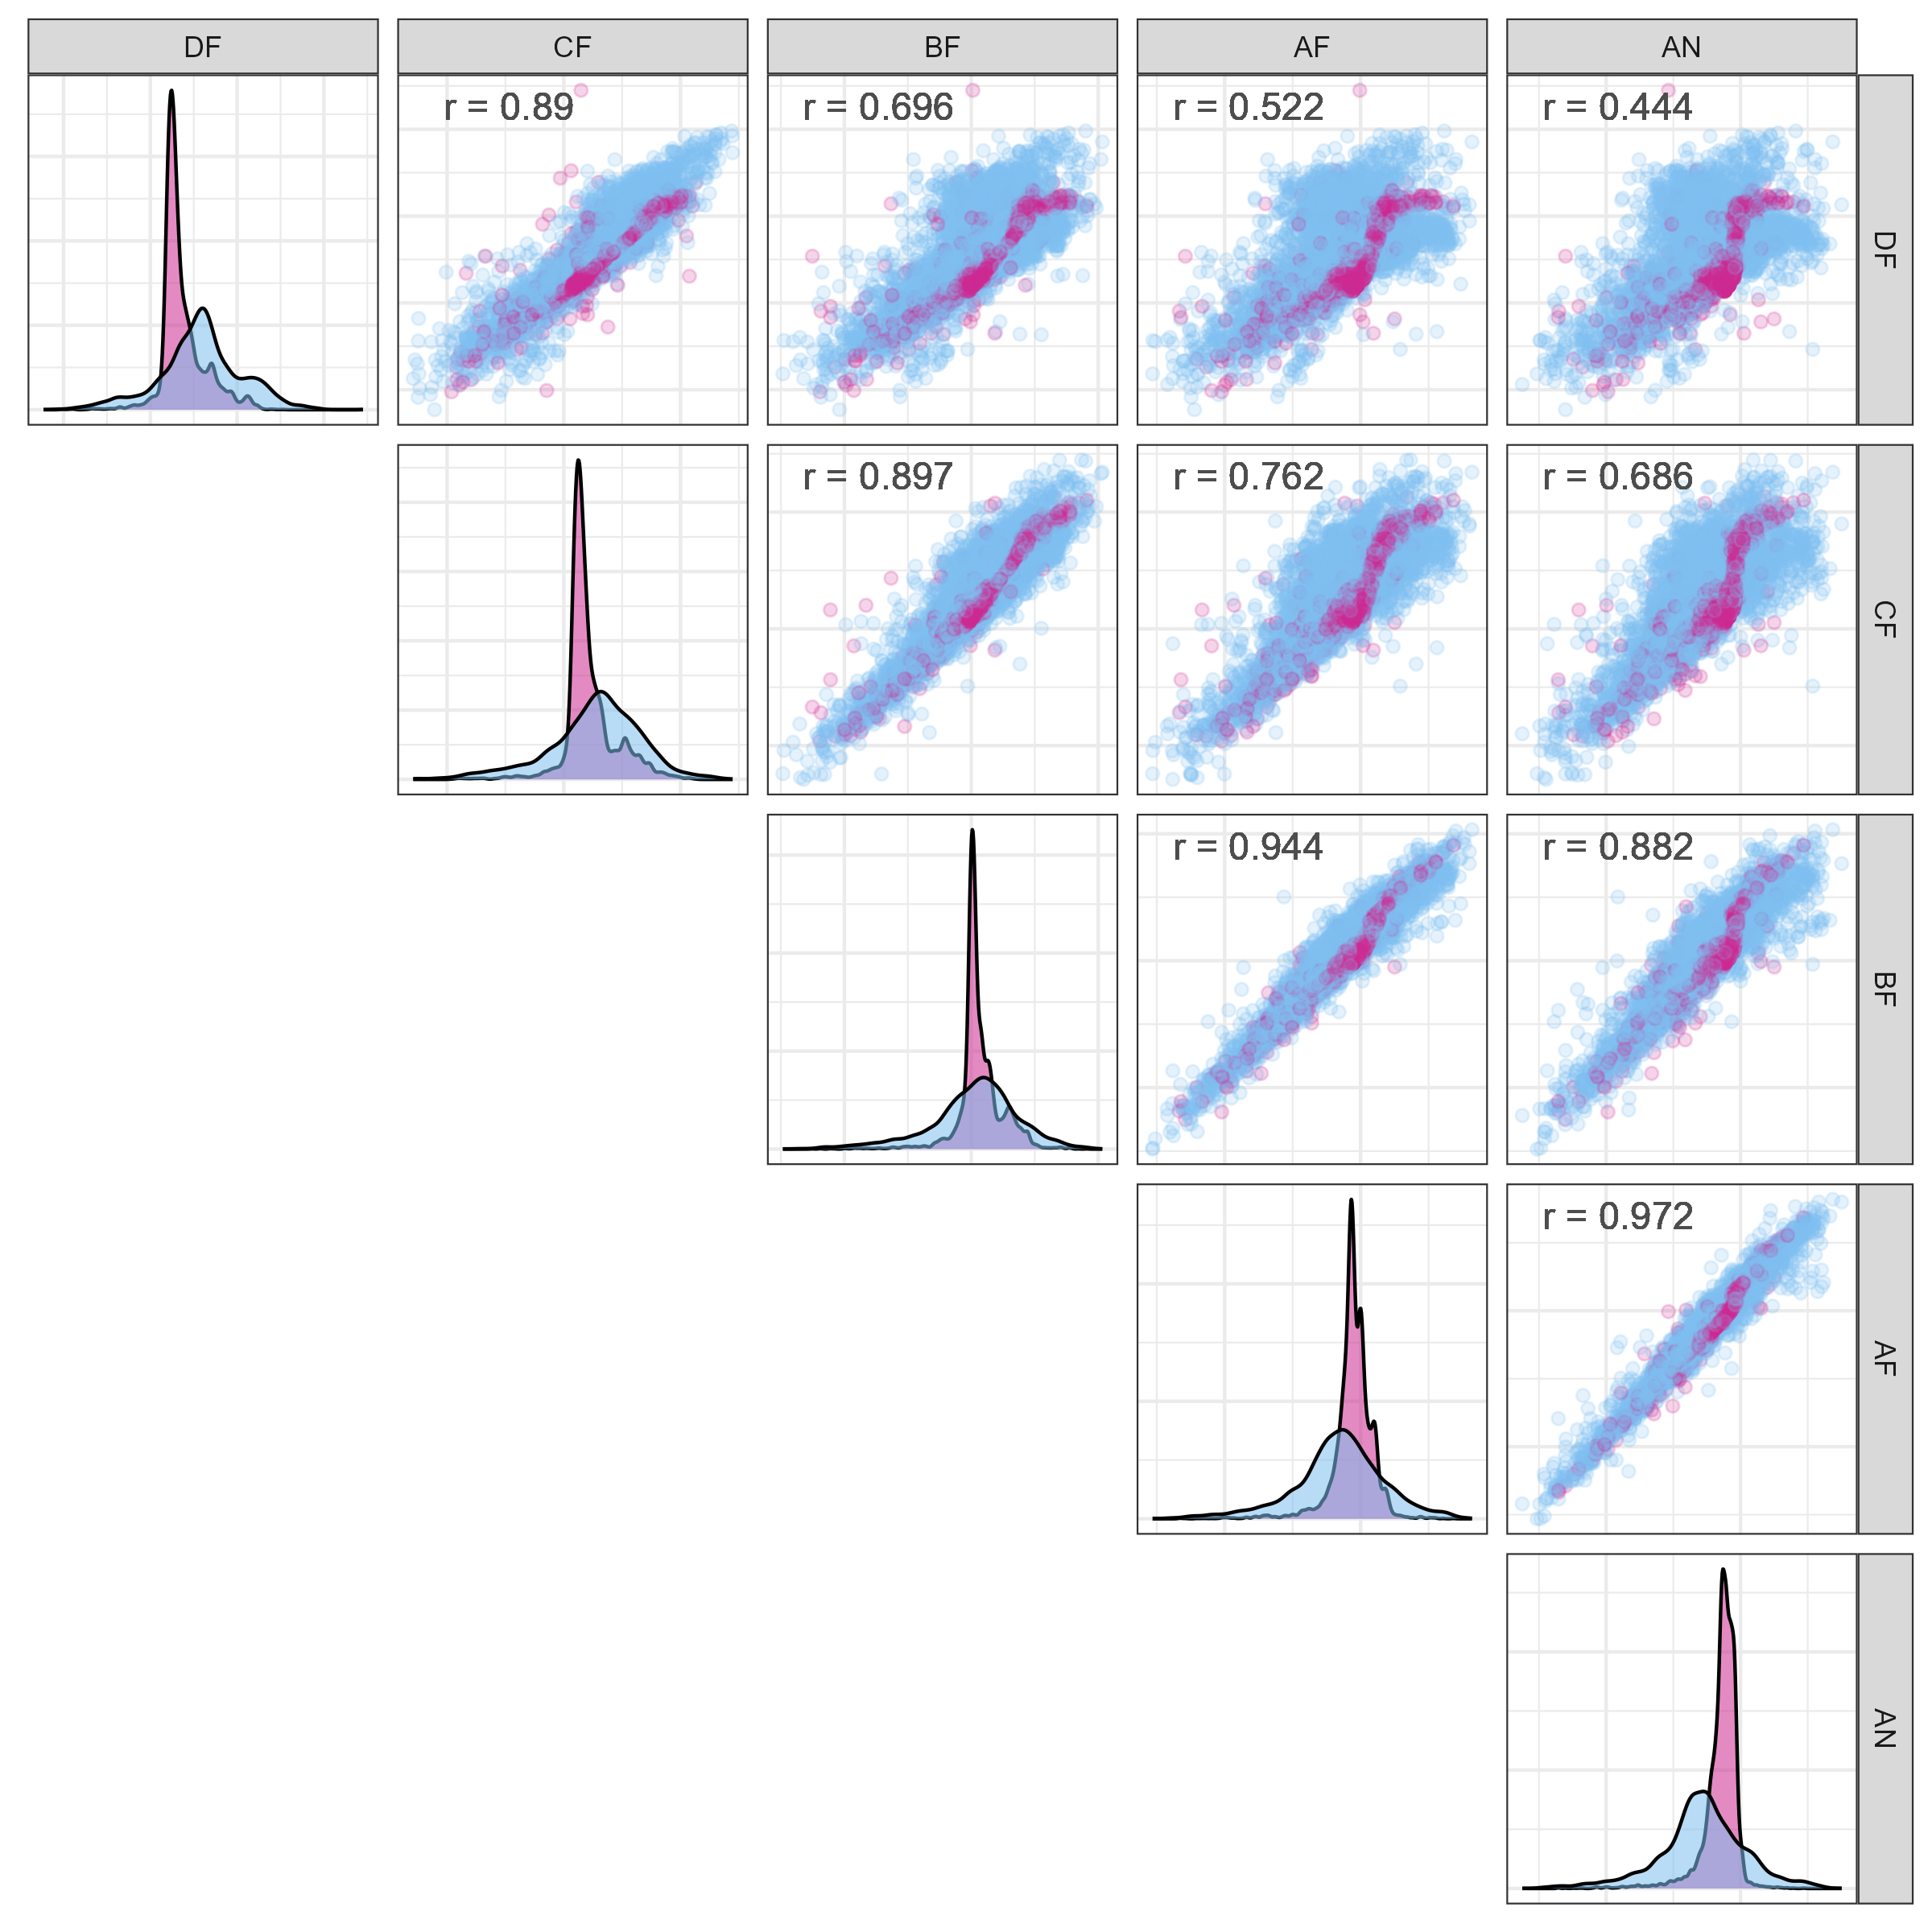
\includegraphics[width=\textwidth]{figs/corr1_void.png}
        \label{subfig:corr1}
    \end{subfigure}
    \hfill
    \begin{subfigure}[t]{0.3\textwidth}
        \centering
        \caption{Image O013257}
        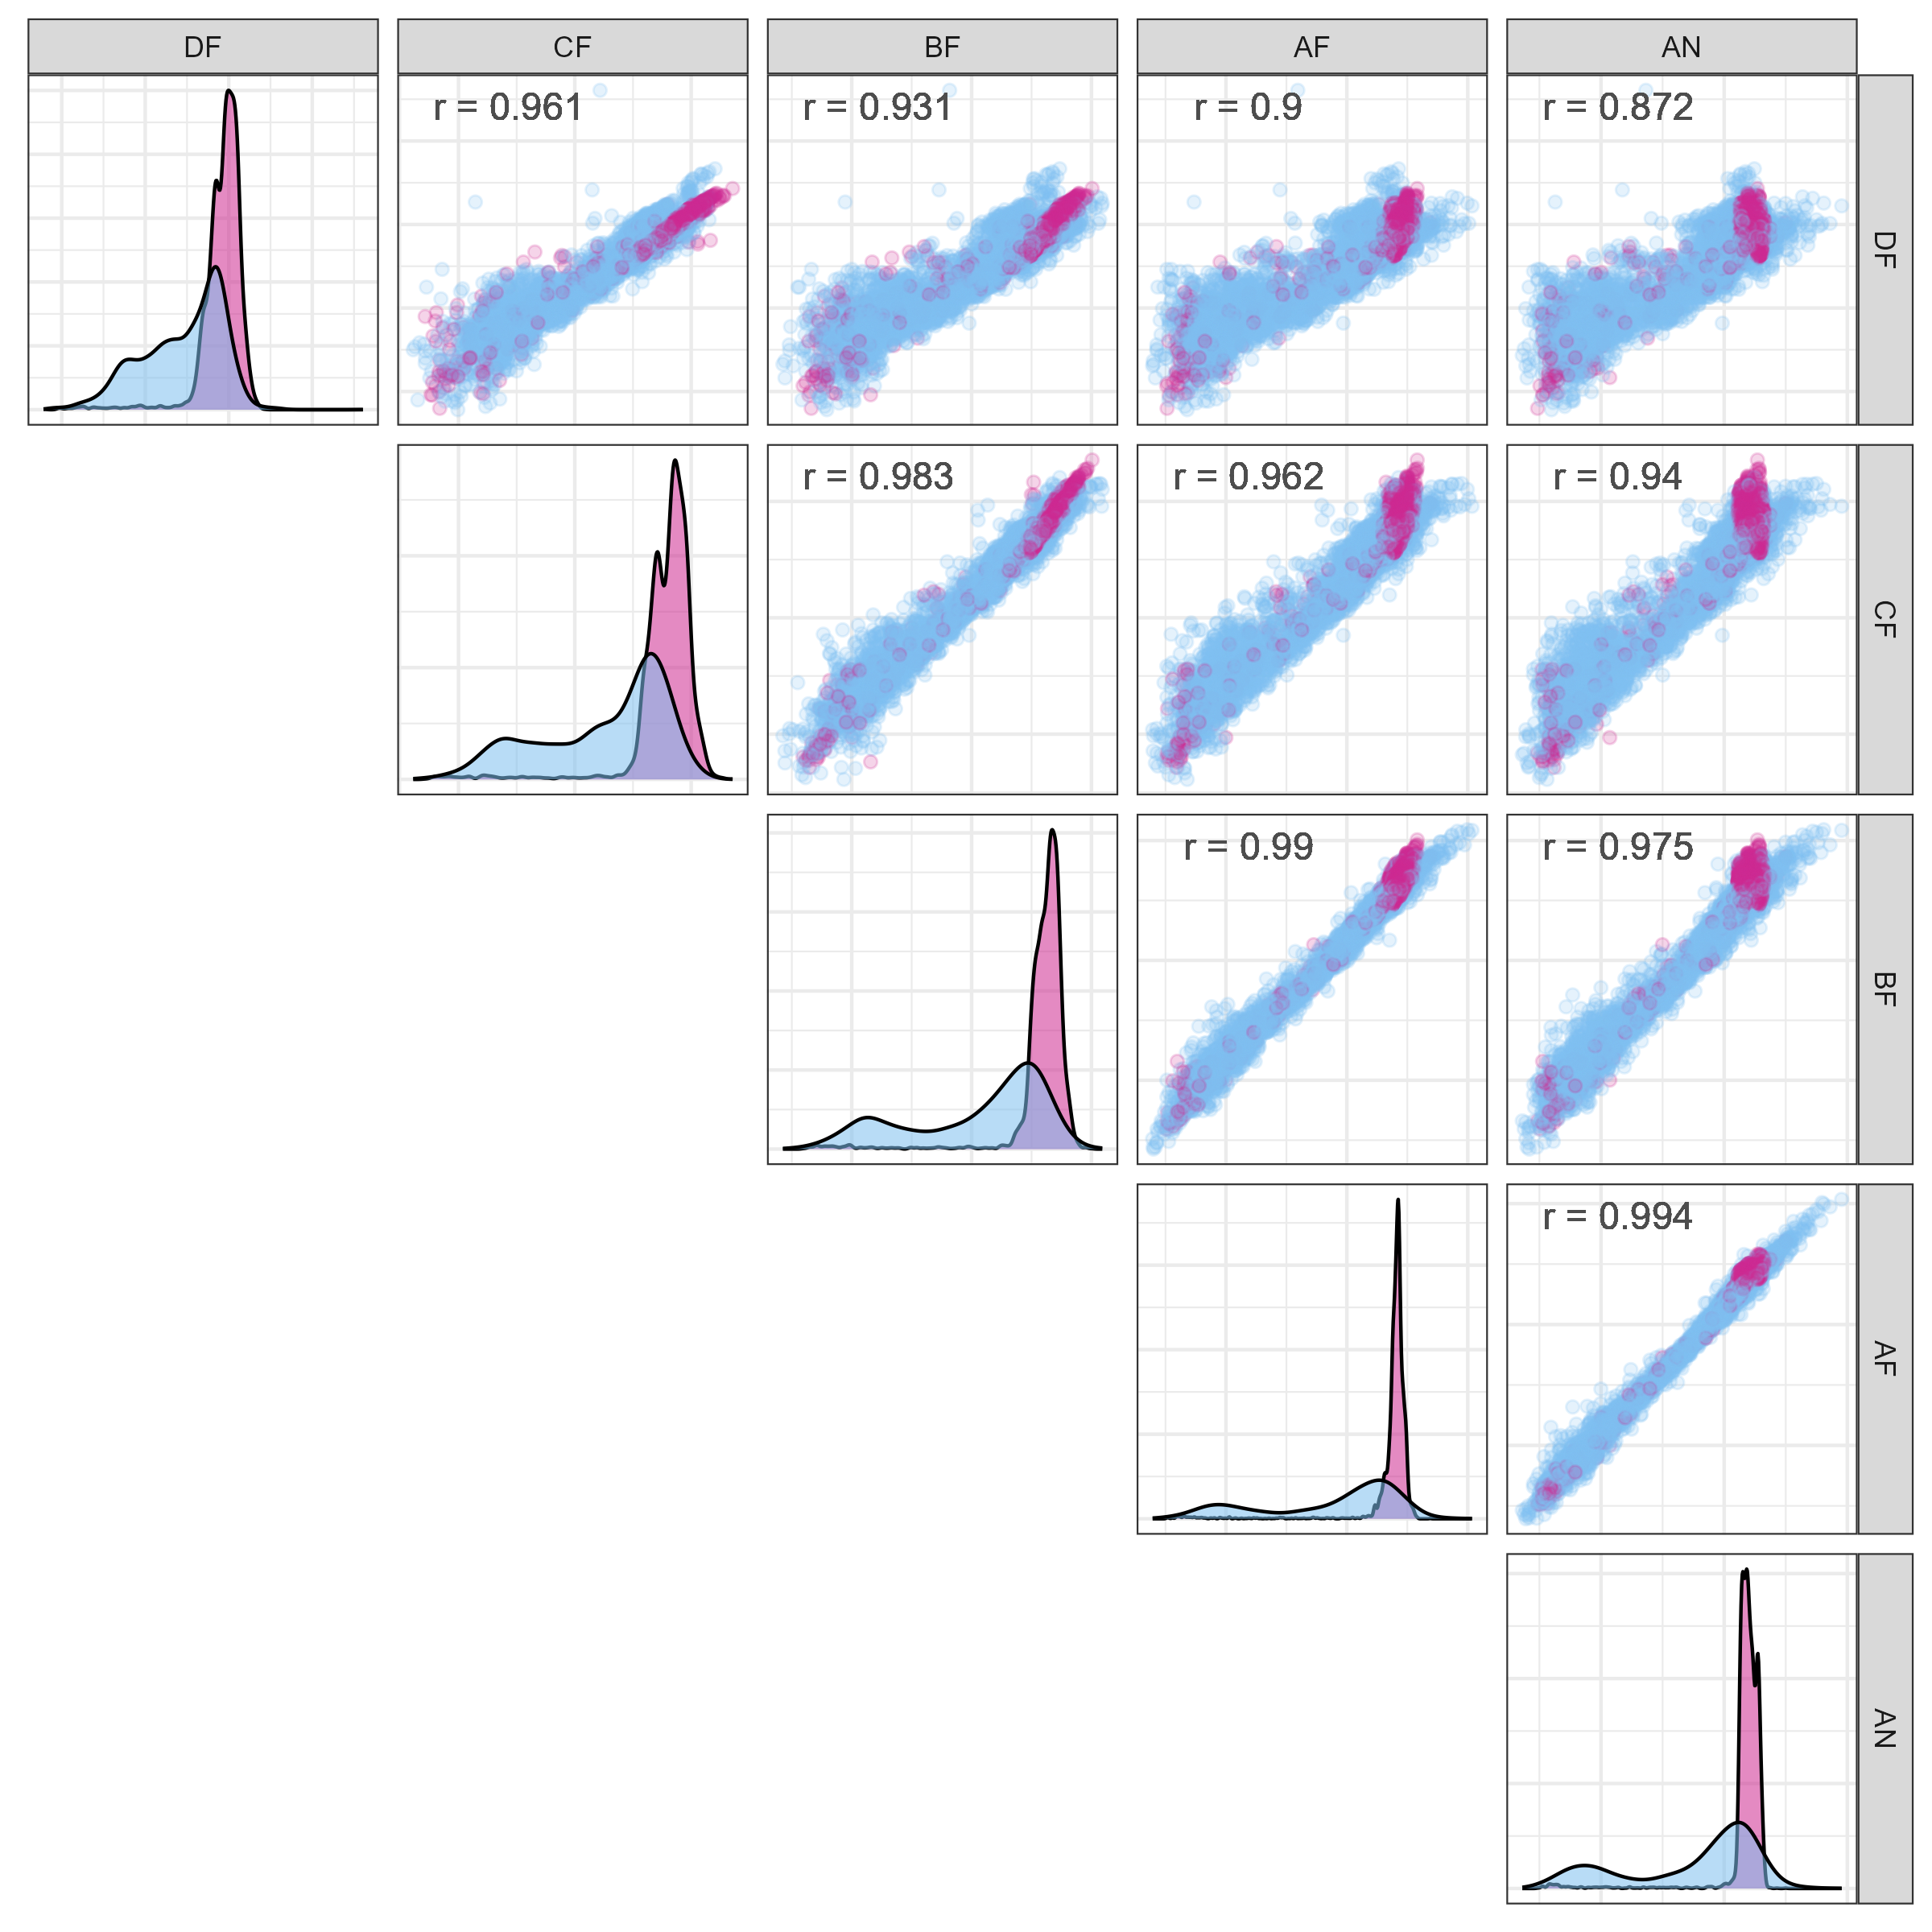
\includegraphics[width=\textwidth]{figs/corr2_void.png}
        \label{subfig:corr2}
    \end{subfigure}
    \hfill
    \begin{subfigure}[t]{0.3\textwidth}
        \centering
        \caption{Image O013490}
        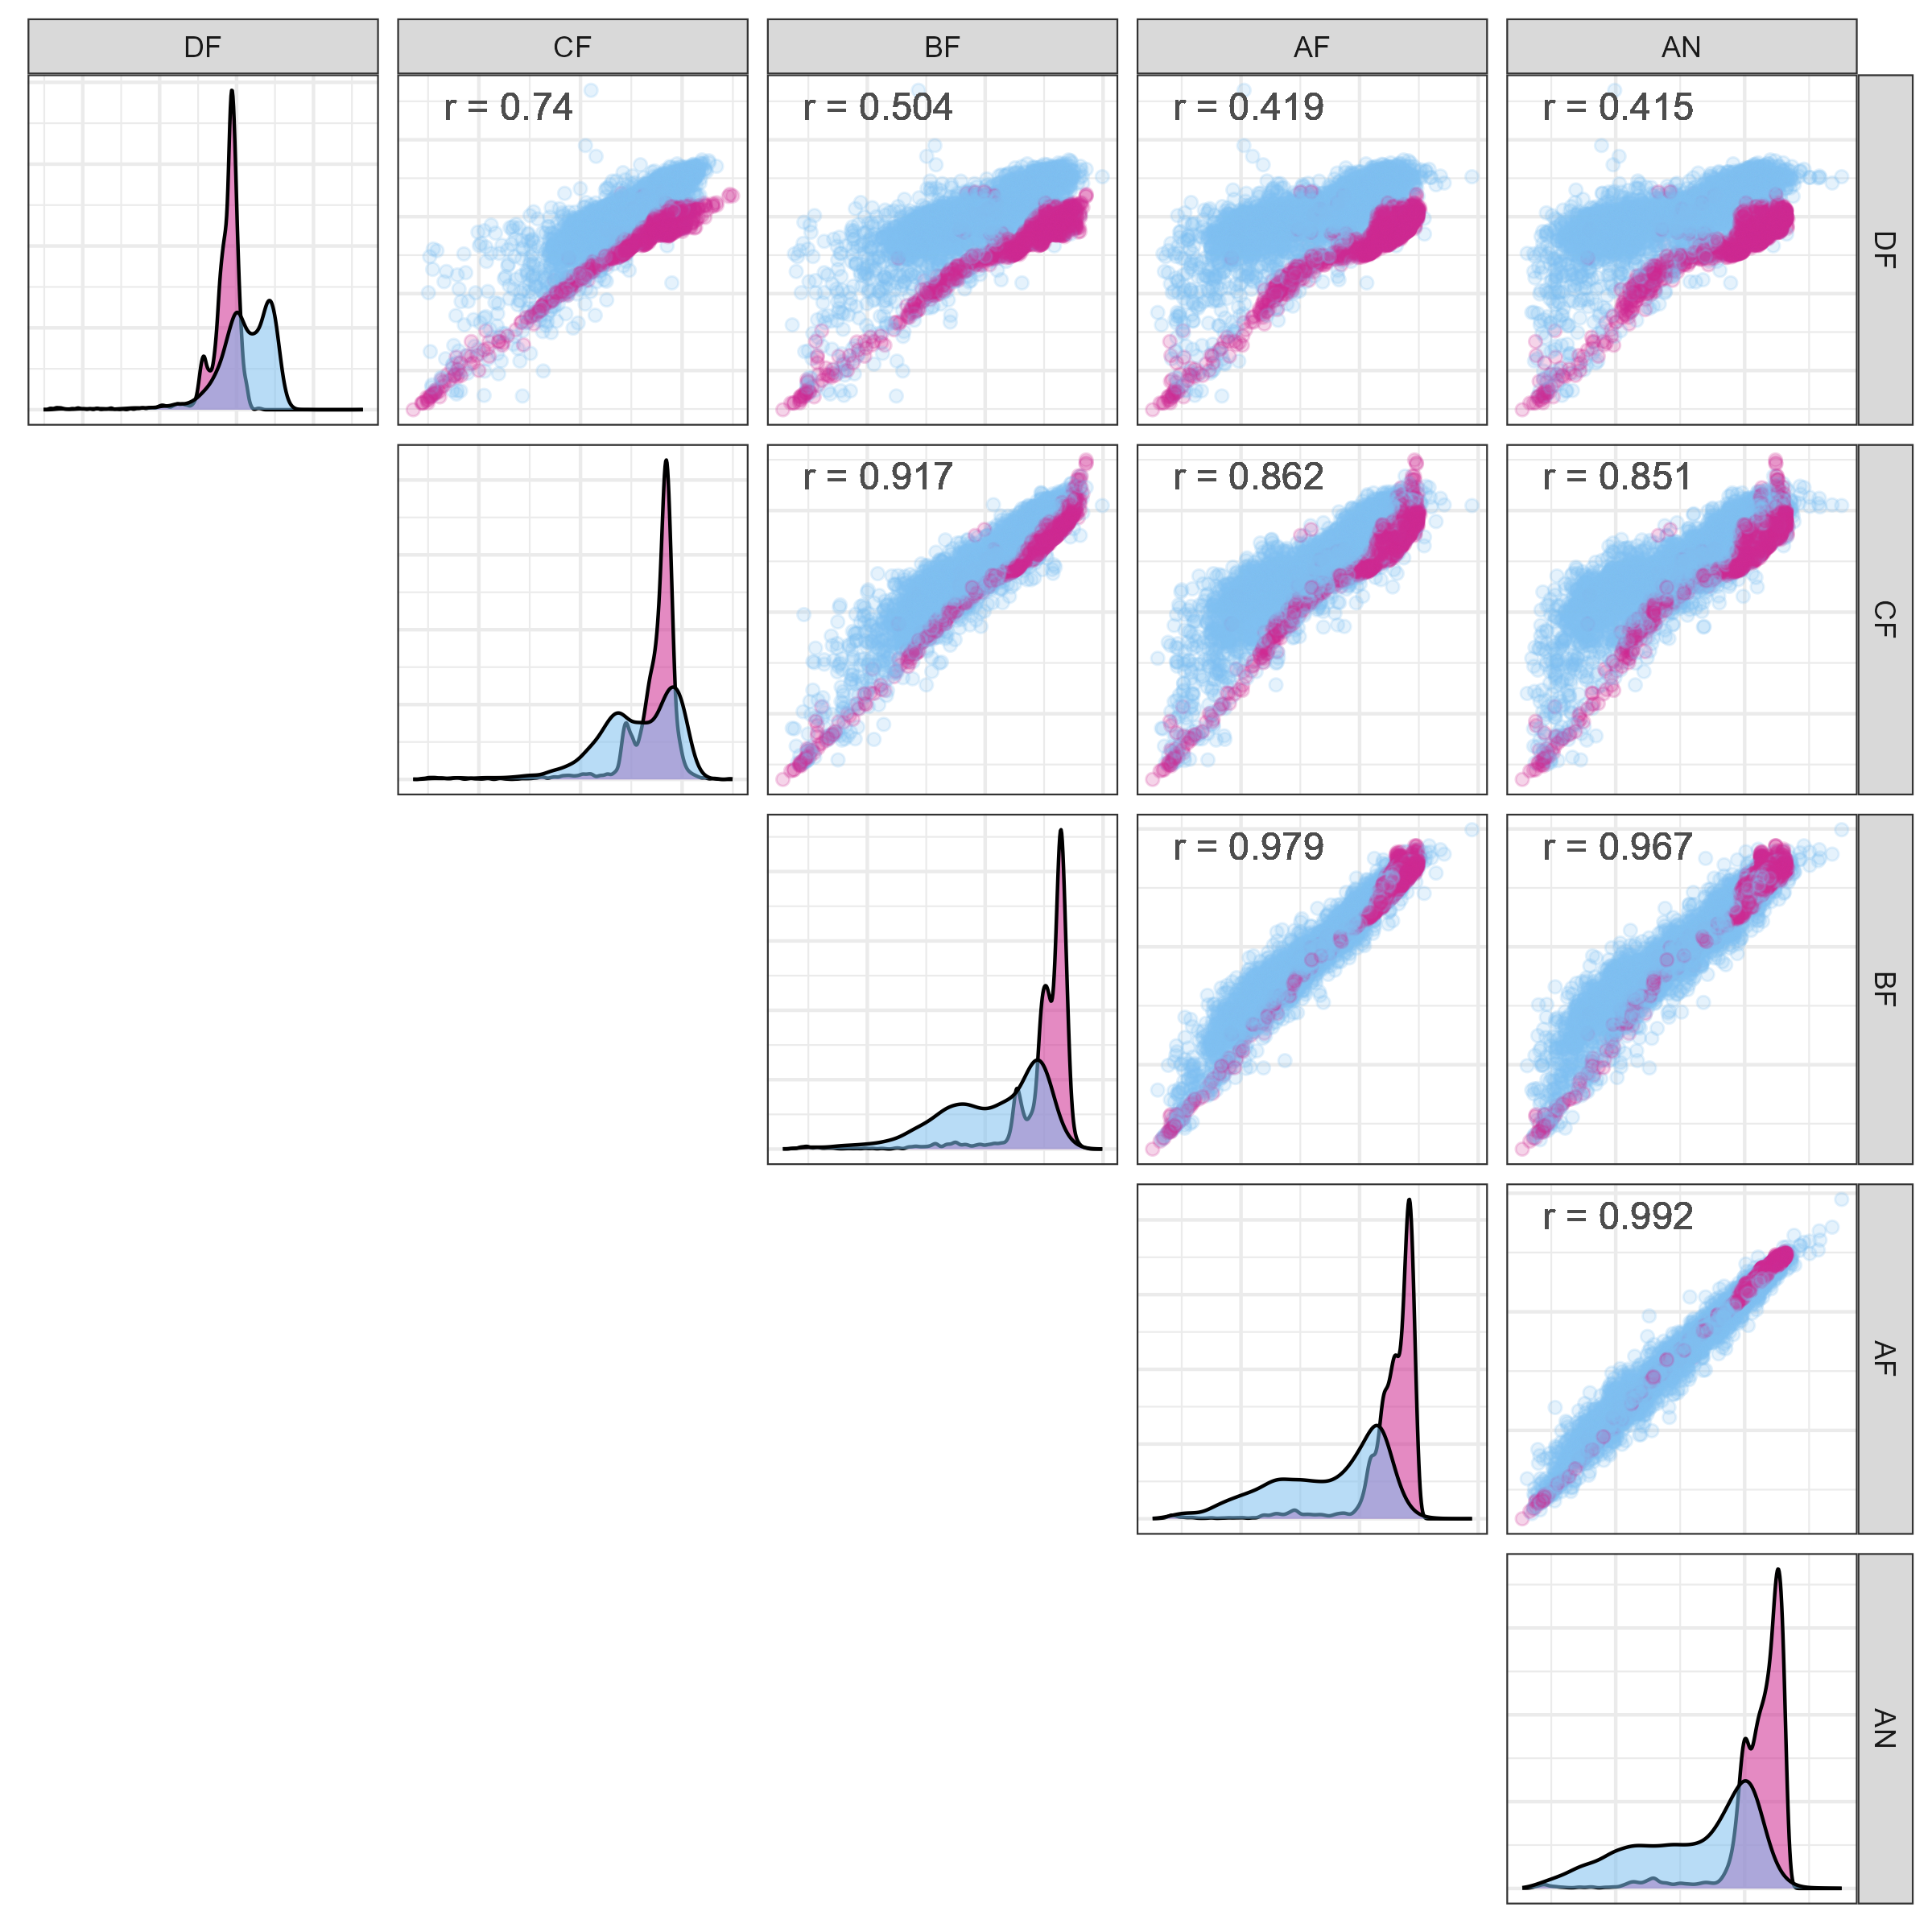
\includegraphics[width=\textwidth]{figs/corr3_void.png}
        \label{subfig:corr3}
    \end{subfigure}
    \caption{Pairwise scatterplots of radiance angles for a balanced sample of $n=10,000$ pixels. Cloud and non-cloud pixels show distinct clustering, suggesting separability, and correlations are generally strong and positive.}
    \label{fig:corr_combined}
\end{figure}

In Figure \ref{fig:corr4}, we present scatterplot matrices for the three constructed features: CORR, SD, and NDAI. Using the same color scheme as before, we plot these scatterplots as a row for each annotated image. Unlike the angular radiances, which exhibited strong linear correlations, these features show only weak to moderate correlations. However, more importantly, we still observe distinct clusters of cloud and non-cloud pixels in each plot. Additionally, the relationships between feature pairs appear consistent across images, suggesting that these constructed features are more stable across time and space than the image-specific clustering seen in the previous figures. This supports previous research identifying CORR, SD, and NDAI as particularly useful for distinguishing between cloud and non-cloud pixels.

\begin{figure}[ht]
    \centering

    % Added title and subtitle to figure
    % and removed them from the subplots
    % corr{N}.png  vs. corr{N}_void.png
    \parbox{\textwidth}{\centering 
        \fontsize{13pt}{13pt}\selectfont \textbf{Scatterplot Matrix of CORR, SD, \& NDAI}  
        
        {\fontsize{11pt}{13pt}\selectfont Comparing equal subsamples of pixels labeled as \textcolor{Cyan}{\textbf{Cloud}} vs. \textcolor{RedViolet}{\textbf{Non-Cloud}}.} 
    }

    \begin{subfigure}[t]{0.3\textwidth}
        \centering
        \caption{Image O012791}
        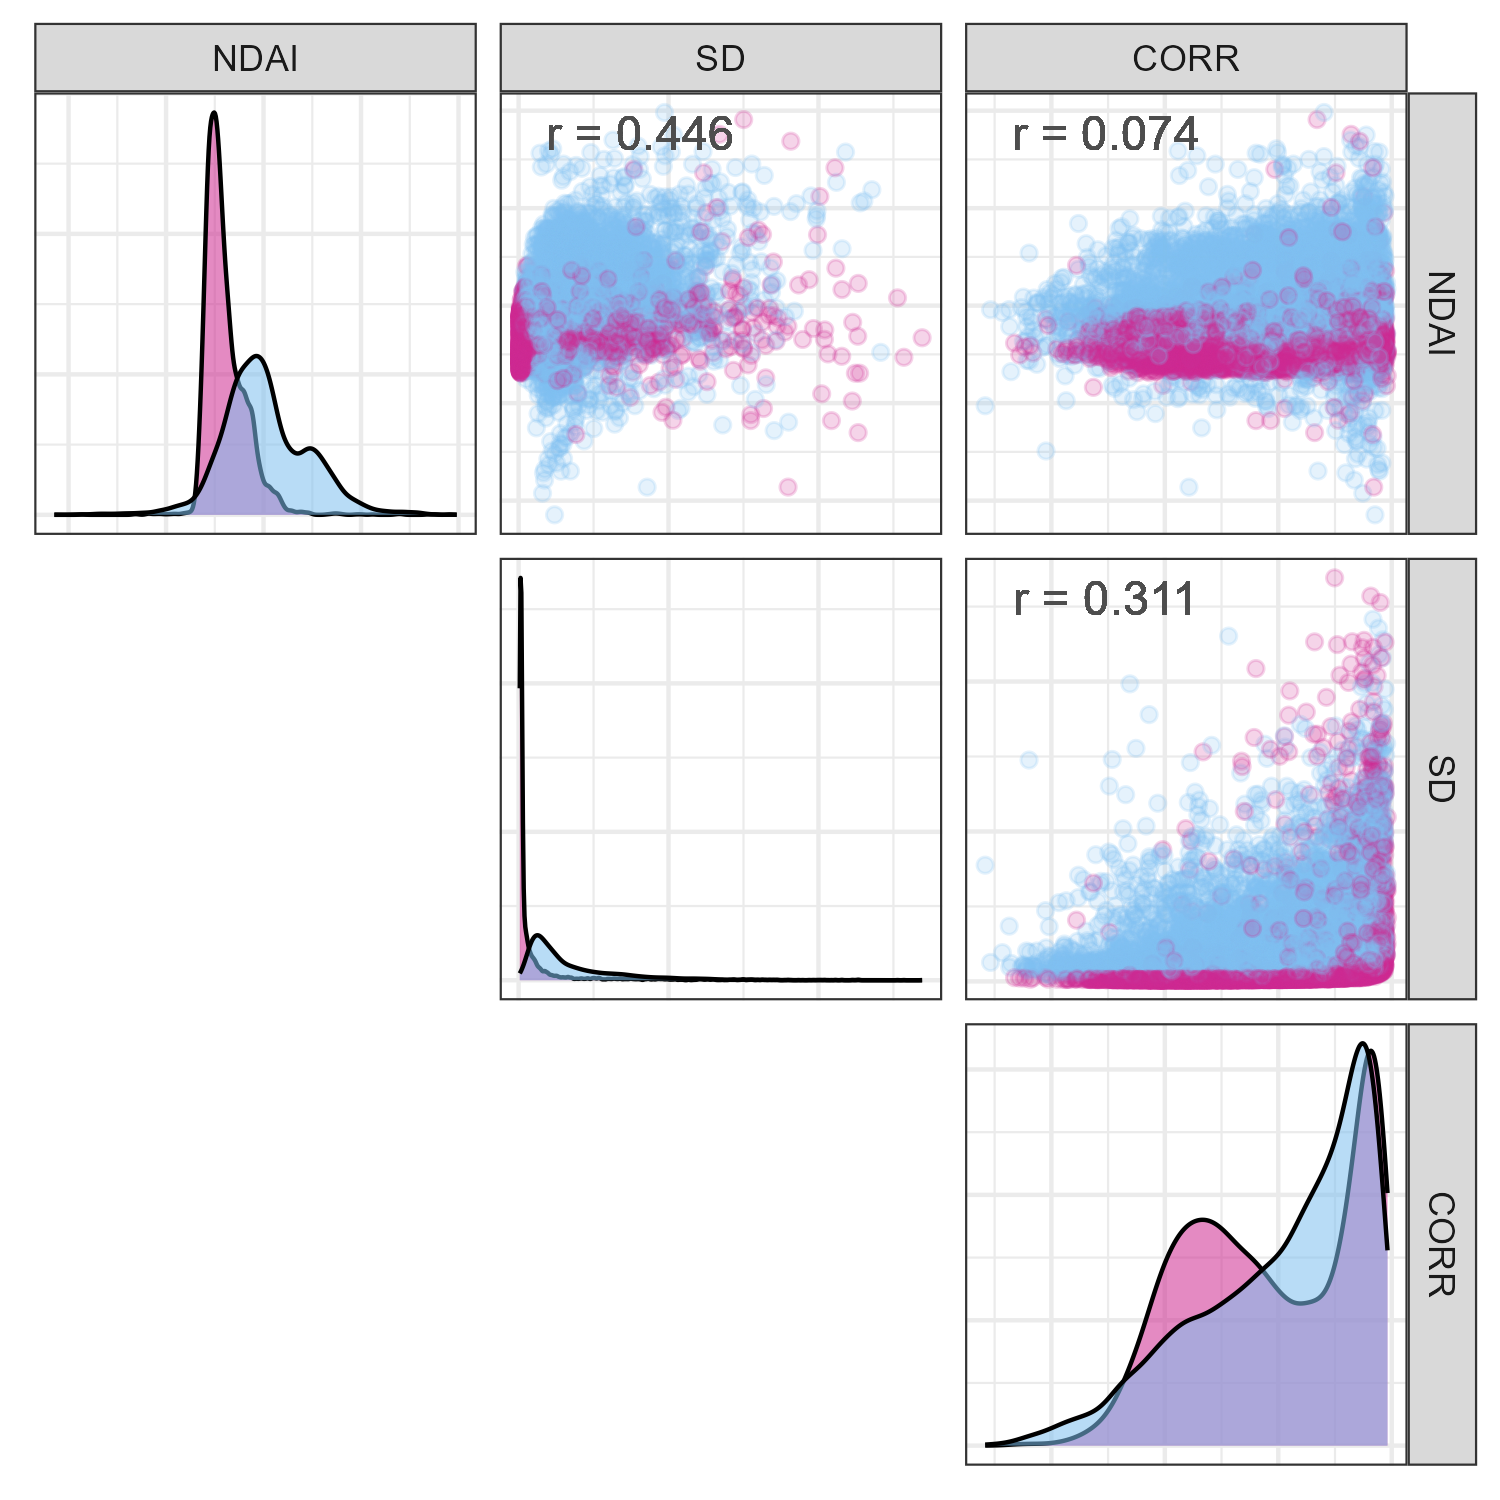
\includegraphics[width=\textwidth]{figs/corr41_void.png}
        \label{subfig:corr41}
    \end{subfigure}
    \hfill
    \begin{subfigure}[t]{0.3\textwidth}
        \centering
        \caption{Image O013257}
        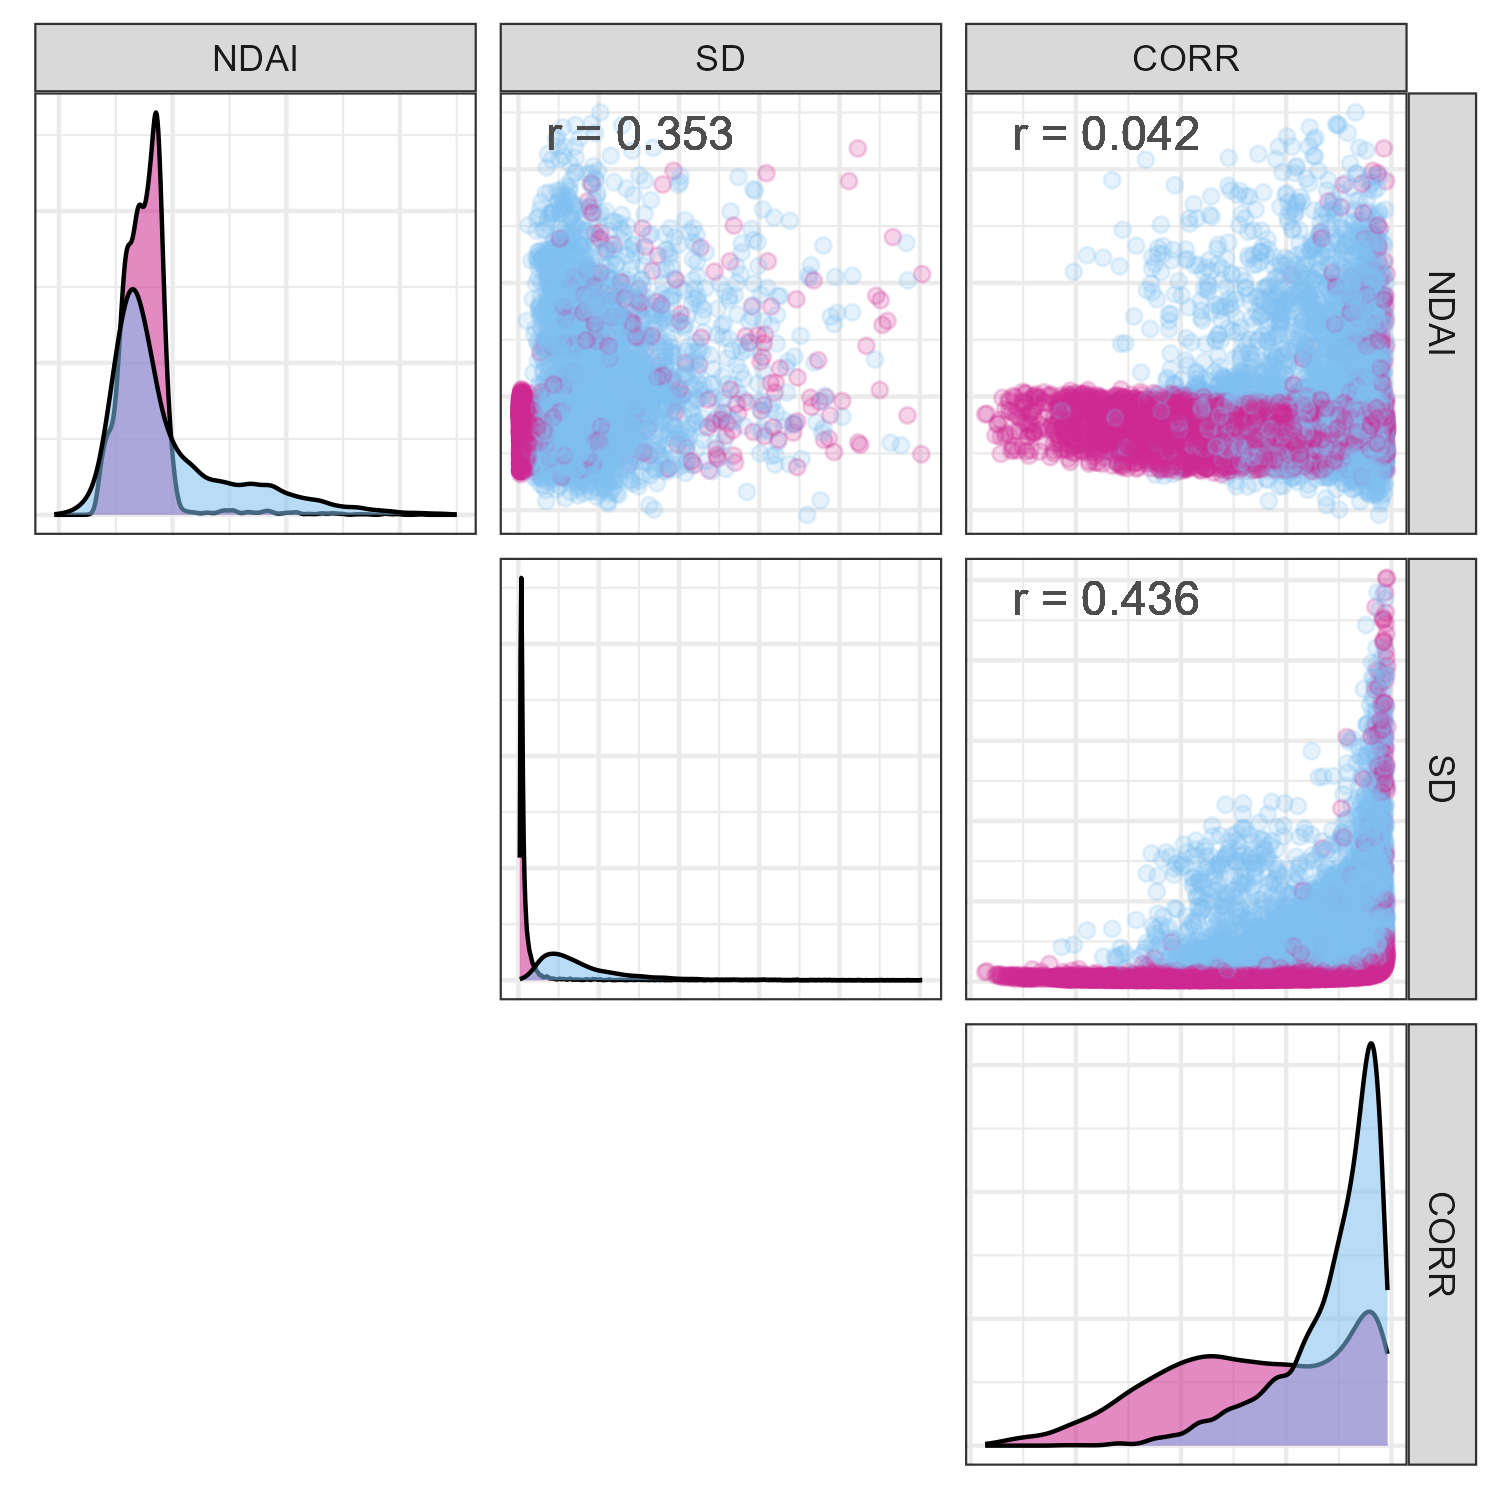
\includegraphics[width=\textwidth]{figs/corr42_void.png}
        \label{subfig:corr42}
    \end{subfigure}
    \hfill
    \begin{subfigure}[t]{0.3\textwidth}
        \centering
        \caption{Image O013490}
        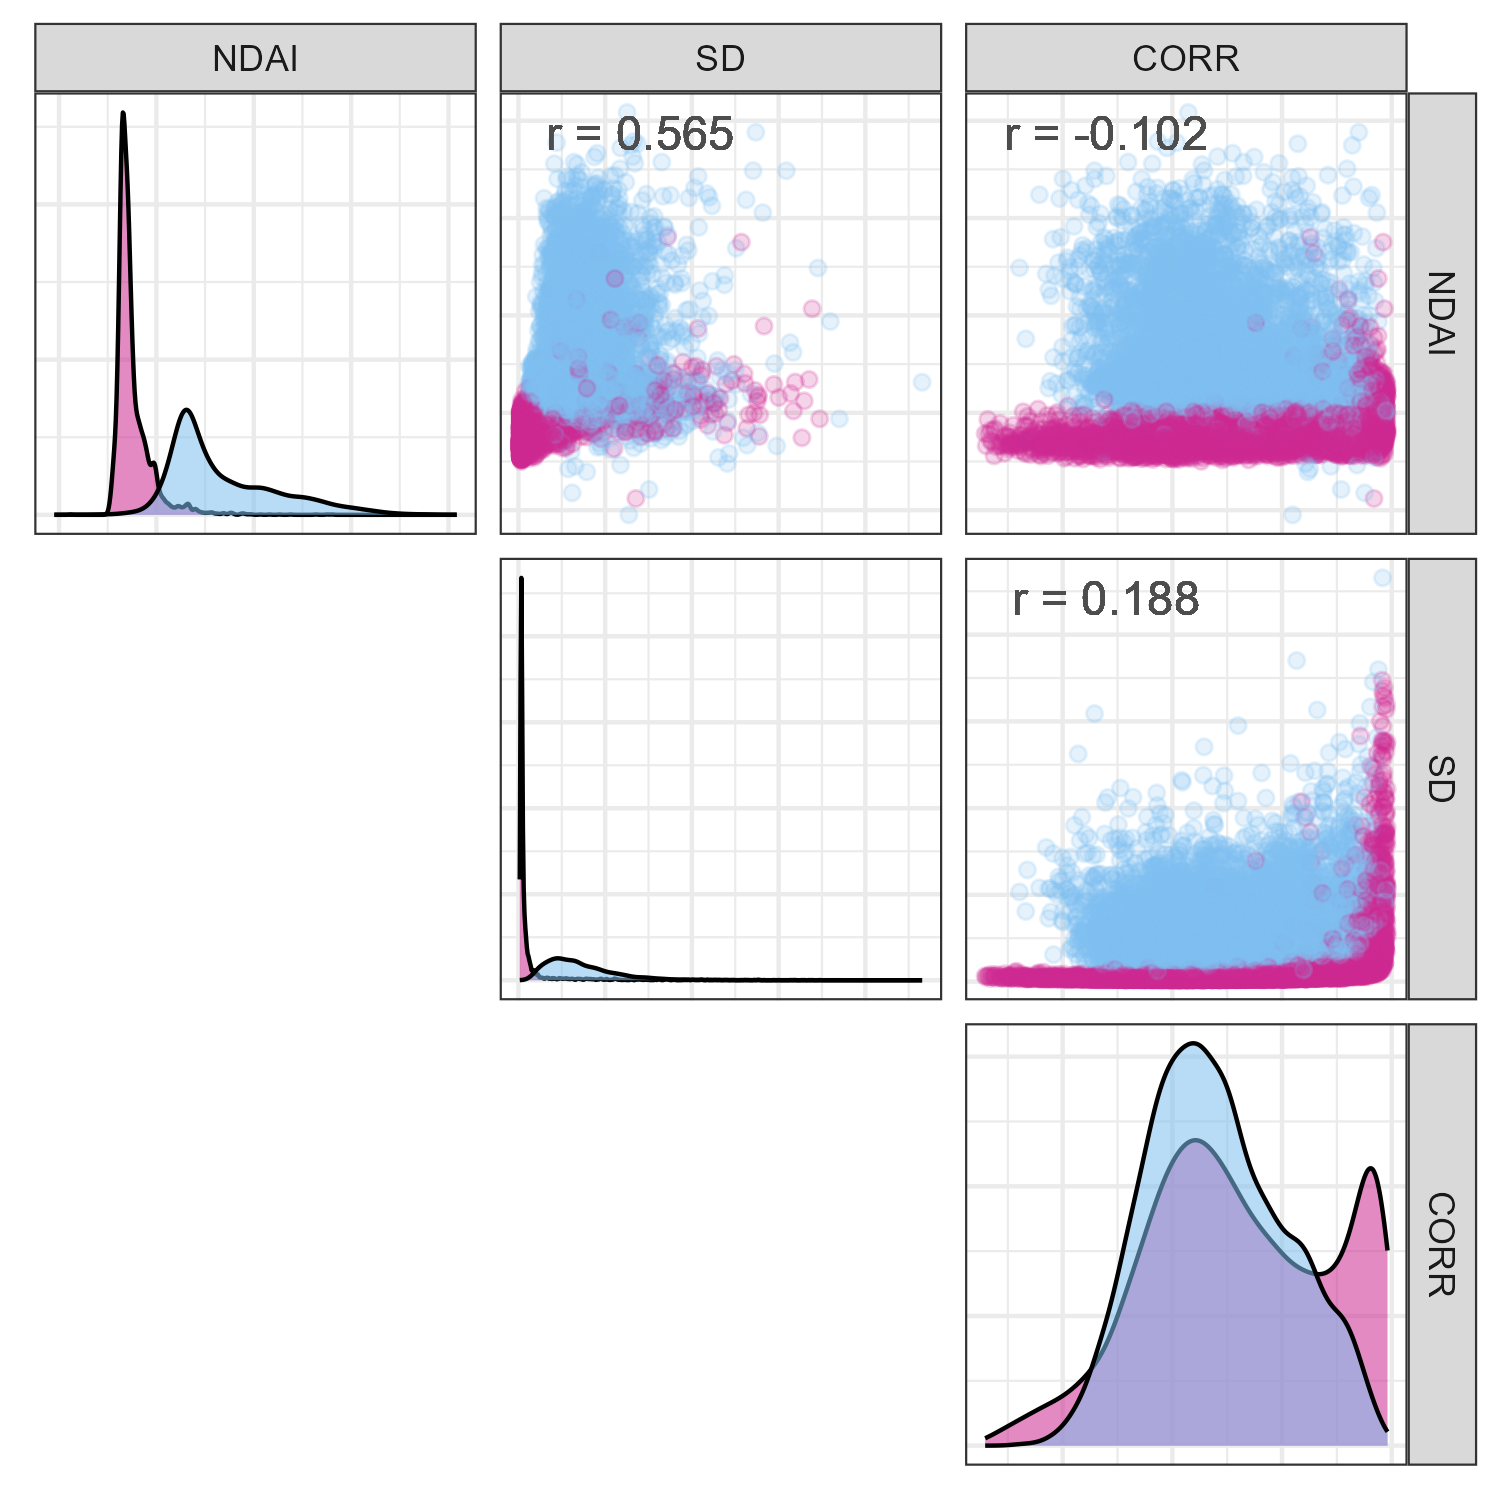
\includegraphics[width=\textwidth]{figs/corr43_void.png}
        \label{subfig:corr43}
    \end{subfigure}
    \caption{Pairwise scatterplots of CORR, SD, and NDAI for a balanced sample of $n=10,000$ pixels. While relationships between variables appear nonlinear, cloud and non-cloud pixels still show distinct clustering.}
    \label{fig:corr4}
\end{figure}

% Old Figure
%\begin{figure}[ht]
%    \centering
%    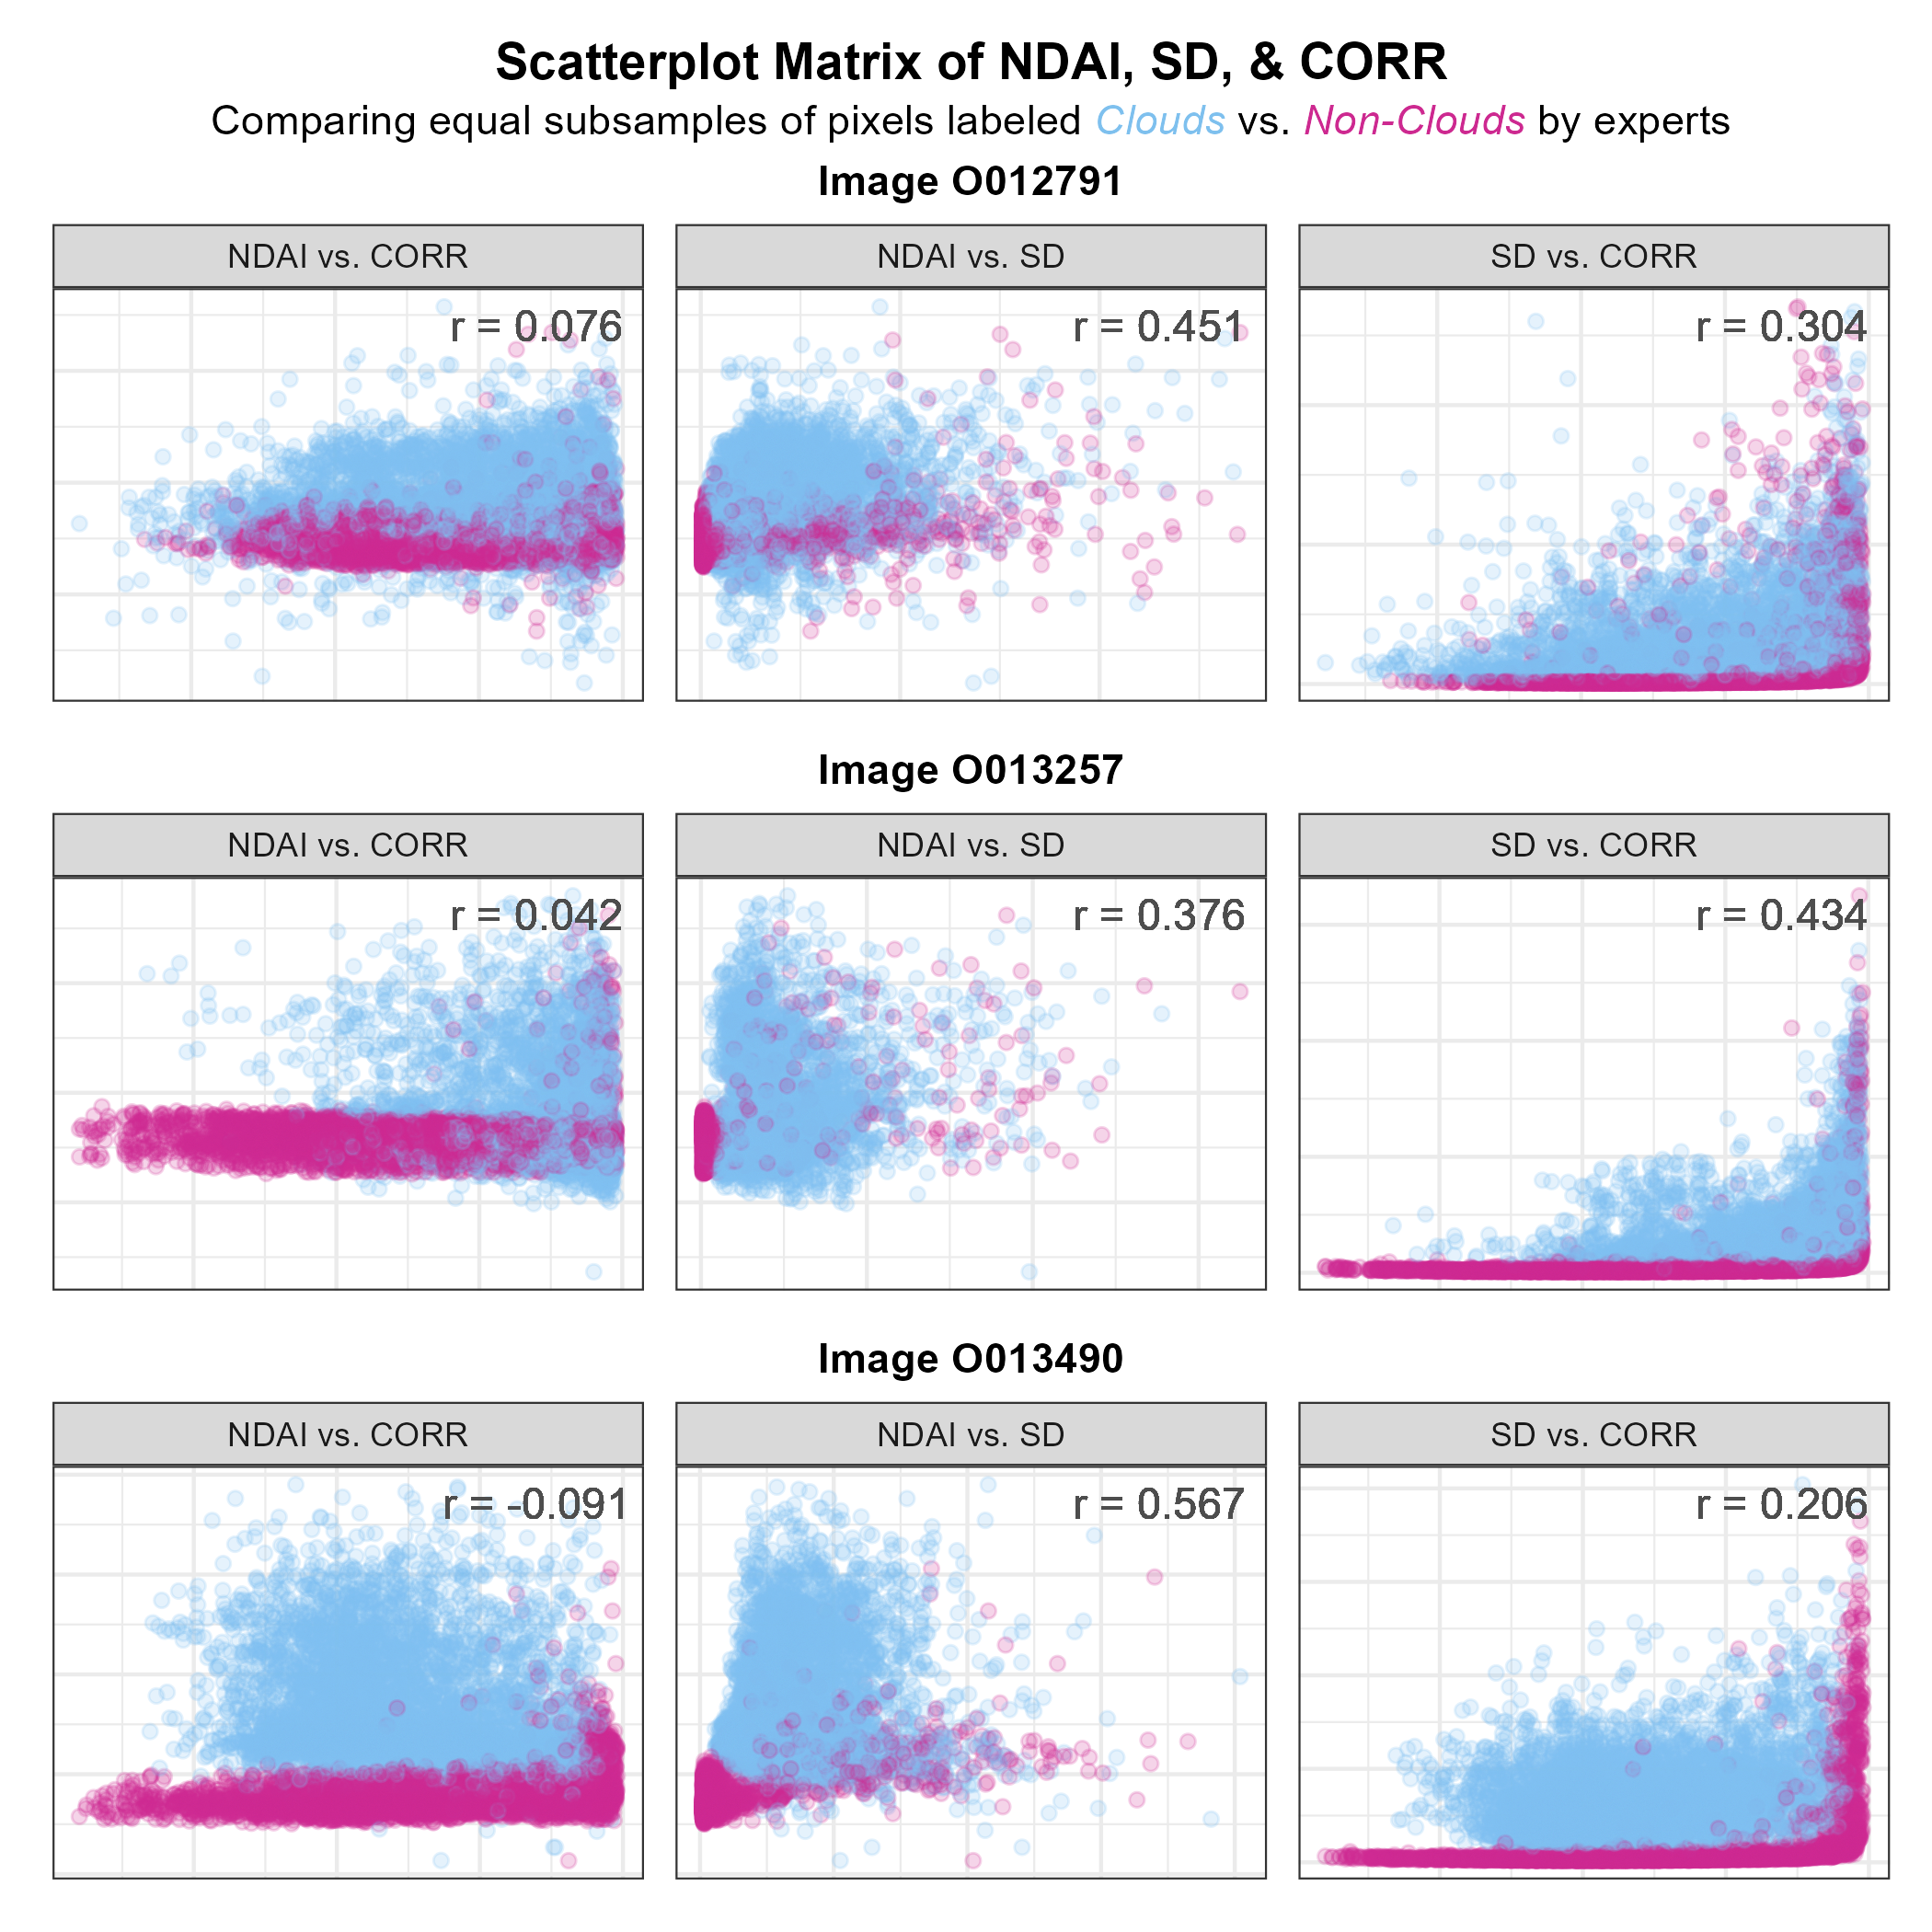
\includegraphics[width=0.5\textwidth]{figs/corr4.png}
%    \caption{Scatterplot Matrix of NDAI, SD, \& CORR}
%    \label{fig:corr4}
%\end{figure}

\subsection{Data Splitting Strategy}

To best mimic real-world applications and ensure generalization beyond spatial correlations within a single image, we split the labeled data at the image level: two images for training and validation (via cross-validation) and one for testing. This approach simulates real-world application to new, unseen images, ensuring generalization beyond spatial correlations within a single image, a critical consideration given the tiny 3-image dataset, because the patterns in different images could be different in terms of position, brightness, and proportion of clouded pixels. Furthermore, we employ 2-fold cross-validation with the two training images, alternating their roles as train and validation sets, for the same reasons.

\subsection{Data Cleaning and Preprocessing}

Considering the 2D image nature of the MISR data, we convert the tabular data into image-like representations with 8 channels by filling the pixels with the corresponding row in tabular data. Some pixels, however, are missing from the tabular data, leading to missing values at the edges of the images. We address this by padding the images with zeros, a common strategy in deep learning. Additionally, these padded pixels are excluded from the loss function and evaluation metrics during both the autoencoder training and the downstream classification, to avoid biasing the model.

The noise, which is unavoidable in real-world data, is not obvious in the MISR images, so we do not apply any noise reduction techniques that may introduce bias. Furthermore, deep learning models are robust to noise. We also do not observe any significant outliers in the data that would require special treatment, according to the EDA.

\section{Feature Engineering}
% Some of the features might be better predictors of the presence of clouds than others. Assuming the expert labels are accurate, use data analysis to identify and justify three of the most informative features. Provide both quantitative metrics and visualizations to support your selection. Note that while this analysis helps understand feature importance, you are not restricted to using only these features in your classification models.

% Task importance perspective: Use a lightweight CV-tuned RF model to get feature importance.

% Domain knowledge perspective: Why does the original paper choose and construct these features? (Device on the satellite, the ground is more smooth, the cloud is more textured, etc.)

% Based on this information, can you engineer any new features? For example, the three features NDAI, SD, and CORR were created using expert knowledge, but they may not take full advantage of the information contained in surrounding pixels. Perhaps you could create and try some new features that use a patch of data around a point?

% Purpose some new features and explain why they might be useful based on domain knowledge. Add them to the RF model and see if they improve performance. Potential candidates: filter (Like Gaussian) selected channels and append them to the original features to catch spatial information. You can explain them from a denoising perspective.

In this section, we analyze the extracted features from the image data, focusing on their correlation, mutual information scores, and feature importance using a Random Forest classifier. Additionally, we explore newly created texture-based features derived from NDAI.

\subsection{Feature Analysis}

\subsubsection{Mutual Information Scores}

Mutual information is a measure of the mutual dependence between two variables. We calculate the mutual information between each feature and the expert labels to identify the most informative features for cloud detection when they are considered individually. The mutual information scores are shown in Table \ref{tab:mi_scores}.

\begin{table}[ht]
    \centering
    \caption{Mutual Information Scores of Features}
    \label{tab:mi_scores}
    \begin{tabular}{cc}
    \hline
    \textbf{Feature} & \textbf{MI Score} \\ \hline
    SD               & 0.4017            \\
    AF               & 0.2417            \\
    NDAI             & 0.2364            \\
    AN               & 0.2104            \\
    BF               & 0.1843            \\
    DF               & 0.1184            \\
    CF               & 0.1020            \\
    CORR             & 0.0647           
    \end{tabular}
    \end{table}

The high mutual information score of SD aligns with our expectations, as it captures the standard deviation of red-band radiation measurements, which is expected to vary significantly between cloud and non-cloud pixels. However, it only represents the importance of features when they are considered individually, and the interactions between features are not considered.

\subsubsection{Random Forest Feature Importance}

Random Forest importance is another metric to evaluate the importance of features in a classification task. We train a lightweight Random Forest model using cross-validation to measure the feature importance. The top three features based on the Random Forest importance scores are shown in Table \ref{tab:rf_scores}.

\begin{table}[ht]
    \centering
    \caption{Random Forest Feature Importance Scores}
    \label{tab:rf_scores}
    \begin{tabular}{cc}
    \hline
    \textbf{Feature} & \textbf{RF Importance} \\ \hline
    SD               & 0.3001                 \\
    NDAI             & 0.1253                 \\
    CORR             & 0.1151                 \\
    AF               & 0.1101                 \\
    AN               & 0.0942                 \\
    BF               & 0.0936                 \\
    DF               & 0.0845                 \\
    CF               & 0.0733                
    \end{tabular}
    \end{table}

The Random Forest importance scores shows the derived features, SD, NDAI, and CORR, are the most important features for cloud detection. This aligns with our expectations, as these features were specifically designed to capture the contrast observed over Arctic clouds. Compared to the mutual information scores, the Random Forest importance scores consider the interactions between features, providing a more comprehensive evaluation of feature importance.

Notice that a similar feature importance analysis is conducted in the \textbf{Feature Importance Analysis}, and a different ranking is obtained. This discrepancy suggests instability in the overall feature importance ranking, while the \textbf{SD} and \textbf{NDAI} features consistently rank in the top two positions, highlighting their importance in cloud detection.

\subsubsection{Correlation Feature Importance}

Figures \ref{fig:feat_corr} show the correlation between the features. As suggested in the EDA section, the derived features (SD, NDAI, CORR) exhibit weak to moderate correlations, while the angular radiances show strong positive linear relationships. This indicates that the derived features are more independent of each other, and could provide complementary information for cloud detection.

\begin{figure}[ht]
    \centering
    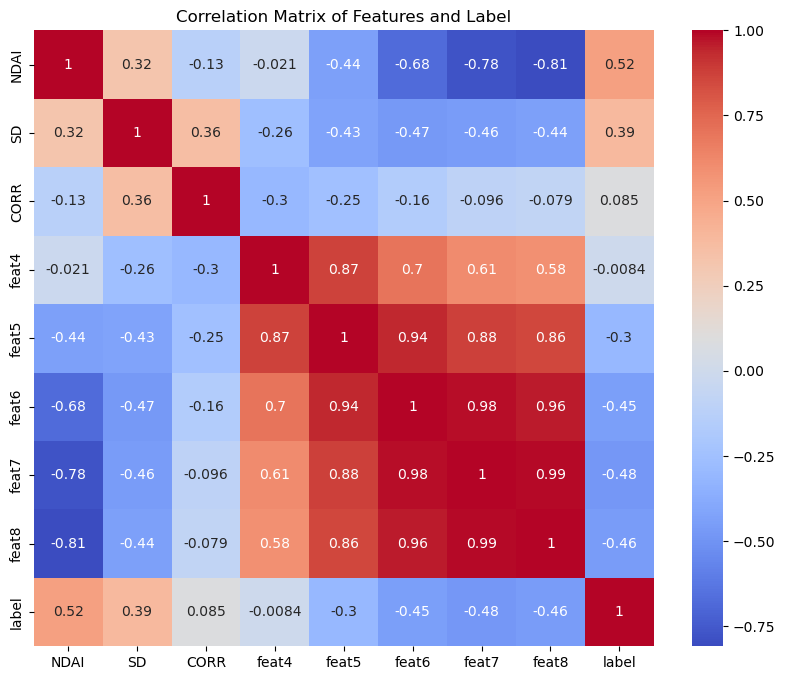
\includegraphics[width=0.8\textwidth]{figs/feat_corr.png}
    \caption{Correlation Matrix of Features}
    \label{fig:feat_corr}
\end{figure}

\subsection{New Feature Engineering}

We consider several new features that capture spatial information in the MISR images, giving the continuous nature of the data and the pixel-wise prediction task. Specifically, we propose the following new features:

\begin{itemize}
    \item \textbf{Contrast}: Measures local intensity variation by computing the difference between maximum and minimum values in a neighborhood window.
    \item \textbf{Homogeneity}: Captures the smoothness of local intensity variations, calculated using variance.
    \item \textbf{Entropy}: Represents the randomness of local pixel intensities using histogram-based entropy calculations.
\end{itemize}

However, due to time constraints and the main focus on the unsupervised representation learning technique, we do not incorporate these new features into the downstream classification models. Nevertheless, we believe these features could provide valuable spatial information and enhance the model's performance in cloud detection tasks.

\section{Representation Learning}
% rephrase the term "transfer learning" to "representation" and explain why it is more appropriate in this context.

% Our model structure choice and limited tuning.

% Training recipes. Why not use the validation set?

Given the limited labeled data (3 images) and the abundance of unlabeled data (161 images), we opt to use a pre-trained model to extract features from the raw MISR images, contrary to the hand-crafted features in the \textbf{Feature Engineering} section. As specified in the instructions, we employ an autoencoder to learn useful representations of the images.

While the lab instructions refer to this process as "transfer learning," we argue that "representation learning" is a more appropriate term in this context. Transfer learning typically involves pre-training a model on a large, general dataset (e.g., ImageNet) and then fine-tuning it on a smaller, task-specific dataset, often with supervised adjustments. In contrast, representation learning emphasizes the unsupervised extraction of useful, abstract features or embeddings from raw data to enhance downstream tasks. This aligns more closely with our approach, where the autoencoder learns a latent representation from unlabeled MISR images to support cloud detection.

For simplicity, we pad all images to 384x384 pixels with 0s, and the pixel values are standardized to have a mean of 0 and a standard deviation of 1 for each channel. All padded pixels are excluded from the loss function.

\subsection{Autoencoder Architecture}

Due to the limited resources and time constraints, we did not test a wide range of backbone architectures for the autoencoder. Instead, we heuristically build an EfficientNet v2-inspired architecture. The more specific design and motivations are as follows:

\begin{itemize}
    \item \textbf{CNN (Convolutional Neural Network) Backbone}: We insist on using a CNN backbone for the autoencoder due to its superiority in capturing spatial information in images. Compared to the patchlization and MLP-based method given in the example, the CNN backbone preserves the spatial structure of the input images, eliminates the hyperparameter tuning of patch size, and avoids the edge effect caused by patchlization.

    \item \textbf{EfficientNet v2-inspired Architecture}: EfficientNet v2 \cite{tan2021efficientnetv2} is the arguably best CNN architecture for general purposes, which incorporates the latest advancements in neural network design and is specifically optimized for fast training and inference on modern hardware. Considering the tiny size of the MISR dataset, we employ the basic building blocks of EfficientNet v2 instead of taking the whole architecture. The basic blocks in Efficient Net v2 are MBConv (Mobile Inverted Residual Block) and Fused-MBConv (Fused Mobile Inverted Residual Block), and the structure of these blocks is shown in Figure \ref{fig:fusedmbconv}.

    \item \textbf{Encoder Structure}: Given the small size of the MISR dataset, which increases the risk of overfitting, we designed a relatively shallow EfficientNet v2-based encoder. The architecture operates in three stages, defined by changes in feature map resolution. The first stage begins with an input convolutional block that transforms the 8-channel input (Padded to 384x384) into 16 channels using a 3x3 kernel with stride 1, preserving spatial dimensions, followed by a Fused-MBConv block that maintains resolution. The second stage applies a Fused-MBConv block with a stride-2 convolution, halving the resolution to 192x192 and expanding to 32 channels. The third stage uses an MBConv block with another stride-2 convolution, reducing the resolution to 96x96, followed by a 1x1 convolution to produce a 64-channel output. To balance capacity and overfitting, we experimented with 1 or 2 repetitions of each block type per stage, adjusting the model's depth as a hyperparameter. The range of the number of parameters is from 35k to 124k. The feature map size is 96x96x64, moderately shrinking the input by 75\% in height and width while expanding the depth by 8 times. This design stems from the low-level nature of the cloud detection task, where the local features are more important than the global context, and an aggressive shrinking of the feature map is not suitable for the pixel-wise prediction task.

    \item \textbf{Decoder Structure}: As its prevalence, we employ an asymmetric and less complex decoder for reconstruction, to prevent the encoder from just learning an "identifier" feature while the autoencoder memorizes input details. The decoder operates in two stages to upsample the encoder's 96x96x64 output back to the original 384x384x8 resolution. The first stage uses a transposed convolution with a 4x4 kernel and stride 2 to expand from 96x96x64 to 192x192x32, followed by a depthwise 3x3 convolution, and a 1x1 convolution for channel adjustment without activation. The second stage applies another transposed convolution (4x4, stride 2) to upsample from 192x192x32 to 384x384x16, followed by a depthwise 3x3 convolution, and a final 1x1 convolution to output 8 channels matching the input. The number of parameters in the decoder is around 42k.
\end{itemize}

\begin{figure}[ht]
    \centering
    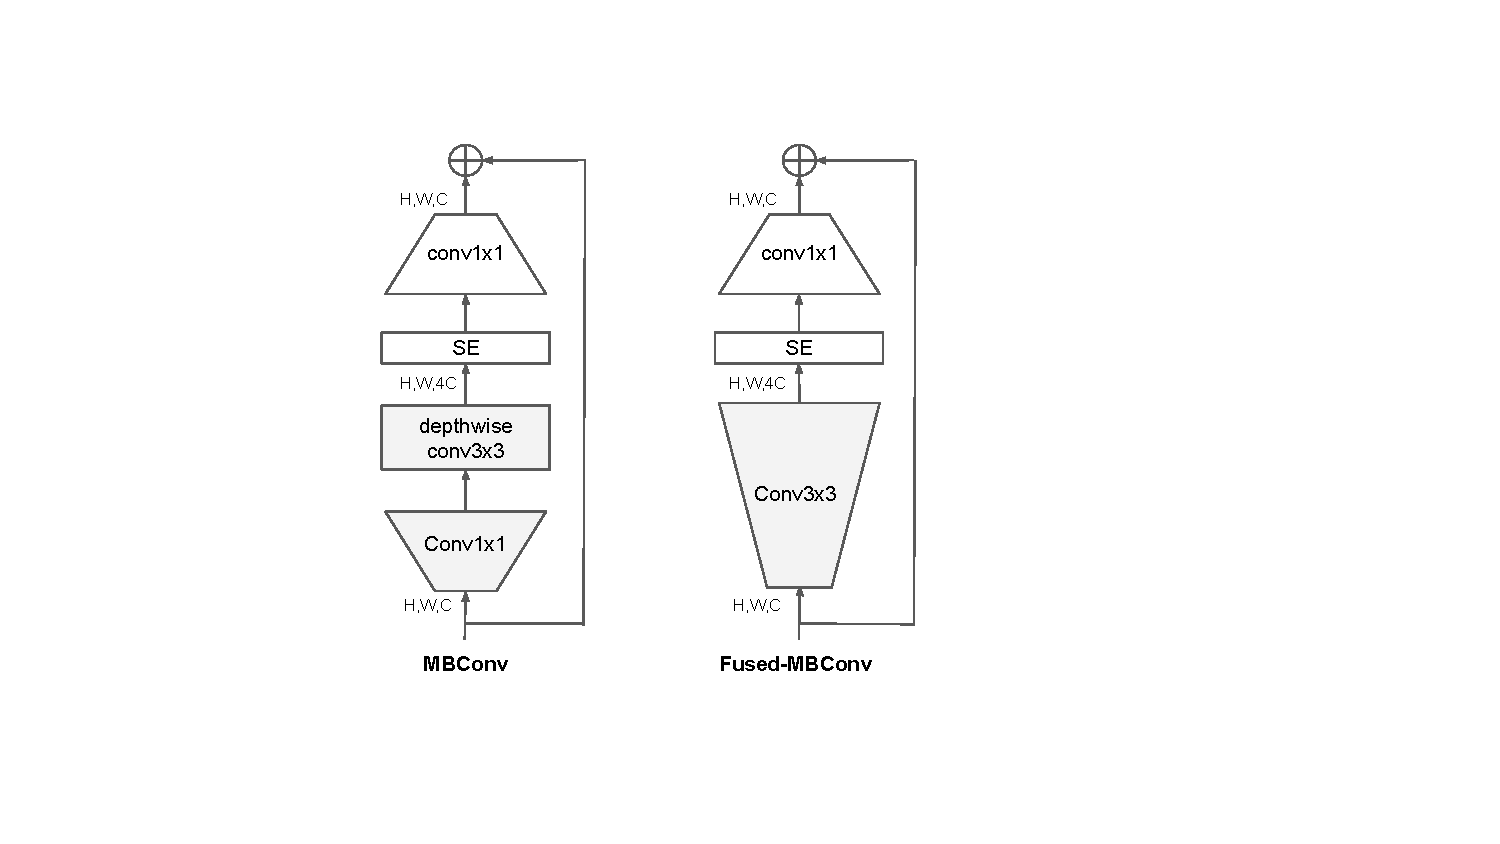
\includegraphics{figs/fusedmbconv.pdf}
    \caption{Structure of MBConv and Fused-MBConv Blocks \cite{tan2021efficientnetv2}}
    \label{fig:fusedmbconv}
\end{figure}

\subsection{Training Recipes}
The standard training recipe for the neural networks is used in this project, including the following components:

\begin{itemize}
    \item \textbf{Loss Function}: We use the MSE to measure the difference between the input and the output of the autoencoder. The reason for choosing MSE includes not much domain knowledge about the MISR images, and the pixel-wise prediction task calls a pixel-wise loss function. The MSE loss is also the default choice for image reconstruction tasks in autoencoders.
    
    \item \textbf{Data Augmentation}: Augmentation is applied to the training set to increase the diversity of the training data and improve the model's generalization ability. As the low-level nature of the cloud detection task and the lack of domain knowledge about "what should be invariant in a MISR image," we apply augmentation conservatively. Only random flipping and rotation are used, and we train different models without augmentation, with one augmentation, or both augmentations to see its effect.
    
    \item \textbf{Optimization}: We use the AdamW optimizer with a learning rate 1e-3 and weight decay 1e-2, and the learning rate is cosine decayed. Full-batch training is used due to the small size of the dataset. We set the number of epochs to 40000, a very large number, but also saved the model during training to mimic the early stopping mechanism.
    
    \item \textbf{Training and Validation Split}: We use all 161 unlabeled images for training and no validation. We claim that reconstruction loss may not be a good proxy for the downstream task performance, so we do not need to use the validation set to tune the hyperparameters, which also reduces the data available for training.
    
\end{itemize}

With the above training recipe, we trained 32 models with 1-2 repetitions of each block type per stage, with or without each augmentation, and for each model, we saved the checkpoints at [100, 200, 400, 800, 1600, 3200, 6400, 12800, 15000, 20000, 25000, 30000, 35000, 40000] epochs. The total number of checkpoints is 448. This is a fairly large number of models and checkpoints, but it is affordable due to the small size of the dataset and the lightweight architecture.

\subsection{Autoencoder Evaluation}

As argued before, we do not measure the performance of the autoencoder in the representation learning stage because we have a straightforward and unique downstream task, which is cloud detection. So we simply leave the evaluation of the autoencoder to the \textbf{Predictive Modeling} section.

\section{Predictive Modeling}
In the \textbf{Feature Engineering} section, we trained simple RFs to measure the feature importance. In this section, we will train several more refined classifiers to predict the presence of clouds, with the original features, the autoencoder features, or the combination of both. The main goal in this section is to achieve a high prediction performance, instead of interpretability or evaluation of the features.

\subsection{Model Evaluation and Selection Criteria}

The ultimate goal of this project is to predict cloud presence in MISR images with high accuracy. However, with only 3 labeled images and significant variation in clouded pixel proportions across them, models trained on this limited data may be biased toward the majority class within each image, which may not reflect the broader dataset's distribution. To mitigate this and enhance robustness, we select the Macro F1 score as our primary evaluation metric and model selection criterion. Macro F1 averages the F1 scores of both classes (cloud: +1, no cloud: -1) equally, encouraging balanced performance across classes despite potential imbalance. Unlike Micro F1, which weights by class frequency, Macro F1 ensures symmetry, as we assume no preference for either class. We also report accuracy as a secondary metric for an intuitive performance overview.

The cross-validation strategy, as described in the \textbf{Data Splitting Strategy} section, is at image-level, to simulate real-world application to new, unseen images.

\subsection{Feature Used}

We consider three types of features for the classification task: the original features, the autoencoder features, and the combination of both. The original features are the raw radiances from the MISR images, while the autoencoder features are the latent representations learned by the autoencoder. The combined features concatenate the original and autoencoder features to leverage both raw and abstract representations. Considering the feature map produced by the autoencoder is 96x96x64, we upscale it to 384x384x64 to match the original padded image size before concatenation and pixel-wise classification.

\begin{table}[ht]
    \centering
    \caption{Cross-Validation Model Performance with Different Features.}
    \label{tab:cv_performance}
    \begin{tabular}{cccc}
    \hline
    \textbf{Model}                 & \textbf{Features}                & \textbf{Macro F1 ± STD} & \textbf{Accuracy ± STD} \\ \hline
    \multirow{2}{*}{Random Forest} & Original Features Only           & 0.8532 ± 0.0015         & 0.8849 ± 0.0014         \\
                                   & Autoencoder or Combined          & 0.7965 ± 0.0024         & 0.7954 ± 0.0017         \\
    \multirow{2}{*}{XGBoost}       & Original Features Only           & 0.8539 ± 0.0000         & 0.8880 ± 0.0000          \\
                                   & Autoencoder or Combined          & 0.8064 ± 0.0000         & 0.8635 ± 0.0000         \\
    \multirow{2}{*}{CNN}           & Original Features Only           & 0.7988 ± 0.0262         & 0.8518 ± 0.0186        \\
                                   & Autoencoder or Combined          & 0.9490 ± 0.0037         & 0.9581 ± 0.0033        \\
    \hline
    \end{tabular}
\end{table}

\subsection{Lightweight CNN Head}

A natural choice for the cloud detection task is utilizing a CNN model, one of the few options that can capture spatial information without the need for manual feature engineering. Two options are considered: a lightweight CNN head on top of the representations learned by the autoencoder and fine-tuning the entire autoencoder model. The former is chosen for its simplicity and efficiency, and the latter is avoided due to the risk of overfitting on the relatively large autoencoder model on the small labeled dataset.

The most important assumption of using a CNN head is that the label is determined by both the pixel's features and its neighbors. This assumption is potentially reasonable because a cloud is not a single pixel but a group of connected pixels, leading to spatial correlations in the image. Thus, a CNN head is supposed to make smoother predictions compared to pixel-wise classifiers like RF and Boosting. However, the drawback is that a shallow CNN head may not be able to capture a complex non-linear relationship between the features and the label. As we will see later, the result of the model selection will tell us if this assumption is reasonable.

\subsubsection{Model Structure}

The lightweight CNN head is designed to process 384x384xC feature maps—whether from the original features, the upscaled autoencoder latent representations, or their concatenation—producing pixel-wise binary predictions for cloud (+1) versus no-cloud (-1) classification. The architecture balances simplicity and the capacity to capture local spatial dependencies and is compatible with all three feature types for direct performance comparison. It consists of a sequence of convolutional layers with batch normalization and activation, optionally incorporating residual connections, followed by a final output layer.

The structure begins with an input convolutional layer that transforms the 64-channel input into a specified number of hidden channels, using a configurable kernel size to define the receptive field. This is followed by a variable number of intermediate convolutional layers, each maintaining the same number of hidden channels and kernel size, to progressively refine spatial features. Each of these layers applies a 2D convolution with "same" padding to preserve the 384x384 resolution, followed by batch normalization to stabilize training and a SiLU activation to introduce non-linearity. When the input and output channels match within a layer, a residual connection adds the input to the output. The sequence concludes with a final convolutional layer that projects the hidden channels to a single output channel, yielding a 384x384x1 prediction map, where values are thresholded for binary classification.

The changeable hyperparameters governing this architecture are:

\begin{itemize}
    \item \textbf{Number of Layers}: The total number of convolutional layers, including the input and output layers, adjustable between 1 (just the output layer) and higher values (up to 3 in our experiment) to control model depth.
    \item \textbf{Hidden Channels}: The number of channels in the intermediate layers, tunable (from 1 to 64) to adjust the width of the model.
    \item \textbf{Kernel Size}: The spatial extent of the convolutional filters (e.g., 3x3, 5x5), determining the size of the local neighborhood influencing each prediction.
\end{itemize}

\subsubsection{Training Recipes}

To train the CNN head for cloud detection, we adopt a structured training pipeline. The training process incorporates a hybrid loss function, regularization, and optimization strategies, with several tunable parameters to optimize performance, as evaluated by the Macro F1 score. Below, we outline the key components and their rationale, highlighting adjustable hyperparameters.

\begin{itemize}
    \item \textbf{Loss Function}: We use a weighted combination of binary cross-entropy (BCE) and hinge loss to compute the pixel-wise error between predictions and expert labels. BCE is the default loss function for binary classification, while hinge loss stemming from soft-margin SVMs encourages margin-based separation, potentially enhancing robustness in class imbalance scenarios but may lead to harder optimization. The mixing ratio between BCE and hinge loss is tunable between 0 and 1, where 0 relies solely on hinge loss and 1 on BCE. Additionally, we support class weighting with a "balanced" option—computed as the inverse frequency of valid labels per class—or no weighting, adjusting for potential skew in the 2 training images. Padded pixels and pixels labeled as 0 (unsure) are excluded from loss computation, ensuring only expert-labeled regions (+1, -1) contribute to learning.

    \item \textbf{Regularization}: To mitigate overfitting given the small dataset, we apply both L1 regularization and weight decay. L1 regularization, with a coefficient adjustable between \(10^{-5}\) and \(0.5\) on a logarithmic scale, penalizes the absolute values of the CNN weights, encouraging sparsity and reducing reliance on noisy features. Weight decay, applied through the optimizer and tunable from \(10^{-5}\) to \(1\) (log scale), adds an L2 penalty to the weights, further stabilizing training by constraining model complexity. These dual mechanisms help balance model simplicity and optimization stability.

    \item \textbf{Optimization}: We explore two optimizers—SGD and AdamW (Adam with weight decay). SGD offers simplicity and constant learning rates, while AdamW adapts learning rates per parameter, potentially accelerating convergence on this small dataset but risks overfitting. The learning rate is adjustable between \(10^{-4}\) and \(10^{-1}\) (log scale). Full-batch training is used due to the limited sample size (1 image per fold).

    \item \textbf{Training Duration}: The number of epochs is tunable from 0 to 1000, allowing exploration of early stopping versus full convergence. A higher epoch count risks overfitting but may capture subtle patterns, while a lower count reduces overfitting.

\end{itemize}

\subsubsection{Hyperparameter Search}

We define a comprehensive hyperparameter search space encompassing the choice of autoencoder features and the CNN head architecture. Table \ref{tab:hyperparams} lists all hyperparameters considered in this optimization process.

\begin{table}[ht]
    \centering
    \caption{Hyperparameters for the Lightweight CNN Head Optimization}
    \label{tab:hyperparams}
    \begin{tabular}{cccc}
    \hline
    \textbf{Name} & \textbf{Type} & \textbf{Range} & \textbf{Applicable To} \\
    \hline
    Number of Classifier Epochs & Integer & [0, 1000] & Original, Autoencoder/Combined \\
    Learning Rate & Float (log) & [$10^{-4}$, $10^{-1}$] & Original, Autoencoder/Combined \\
    Weight Decay & Float (log) & [$10^{-5}$, 1] & Original, Autoencoder/Combined \\
    Optimizer & Categorical & \{SGD, AdamW\} & Original, Autoencoder/Combined \\
    Number of Classifier Layers & Integer & [1, 3] & Original, Autoencoder/Combined \\
    Classifier Hidden Channels & Integer & [1, 64] & Original, Autoencoder/Combined \\
    Kernel Size & Integer & [1, 10] & Original, Autoencoder/Combined \\
    Loss Mixing Ratio & Float & [0, 1] & Original, Autoencoder/Combined \\
    L1 Regularization & Float (log) & [$10^{-5}$, 0.5] & Original, Autoencoder/Combined \\
    Class Weight & Categorical & \{Balanced, None\} & Original, Autoencoder/Combined \\
    Autoencoder Block 1 Repetitions & Integer & [1, 2] & Autoencoder/Combined \\
    Autoencoder Block 2 Repetitions & Integer & [1, 2] & Autoencoder/Combined \\
    Autoencoder Block 3 Repetitions & Integer & [1, 2] & Autoencoder/Combined \\
    Augmentation: Flip & Boolean & \{True, False\} & Autoencoder/Combined \\
    Augmentation: Rotate & Boolean & \{True, False\} & Autoencoder/Combined \\
    Autoencoder Training Length & Integer & [0, 13] & Autoencoder/Combined \\
    Include Original Features & Boolean & \{True, False\} & Autoencoder/Combined \\
    \hline
    \end{tabular}
\end{table}

Due to the large number of hyperparameters and their potential interactions, we employ Optuna \cite{optuna_2019}, a hyperparameter optimization framework, to efficiently explore the search space with feasible computational resources. Optuna uses a Tree-structured Parzen Estimator (TPE) algorithm to prioritize promising regions, shrinking the search space over iterations. We set the number of trials to 9000, a relatively high value to ensure thorough exploration and maximize the Macro F1 score as the objective. Table \ref{tab:selected_hyperparams} presents the selected hyperparameters after optimization for the autoencoder feature and original feature configurations, along with their corresponding Macro F1 scores and accuracies from the hyperparameter search. Notice that the "hidden channels" hyperparameter is not applicable when the number of classifier layers is 1.

\begin{table}[ht]
    \centering
    \caption{Selected Hyperparameters for Lightweight CNN Head with Best Macro F1 Scores}
    \label{tab:selected_hyperparams}
    \begin{tabular}{ccc}
    \hline
    \textbf{Hyperparameter} & \textbf{Autoencoder Features} & \textbf{Original Features} \\
    \hline
    Number of Classifier Epochs & 734 & 505 \\
    Learning Rate & 0.08037 & 0.01894 \\
    Weight Decay & 4.99e-05 & 3.81e-04 \\
    Optimizer & AdamW & AdamW \\
    Number of Classifier Layers & 1 & 3 \\
    Classifier Hidden Channels & - & 54 \\
    Kernel Size & 7 & 1 \\
    Loss Mixing Ratio & 0.641 & 0.373 \\
    L1 Regularization & 5.72e-05 & 3.07e-04 \\
    Class Weight & Balanced & None \\
    Autoencoder Block 1 Repetitions & 1 & - \\
    Autoencoder Block 2 Repetitions & 1 & - \\
    Autoencoder Block 3 Repetitions & 1 & - \\
    Augmentation: Flip & False & - \\
    Augmentation: Rotate & True & - \\
    Autoencoder Training Epochs & 1600 & - \\
    Include Original Features & False & - \\
    \hline
    Macro F1 Score & 0.9539 & 0.9201 \\
    Accuracy & 0.9617 & 0.9283 \\
    \hline
    \end{tabular}
\end{table}

The performance of a CNN model is variable due to the randomness in the initialization and the stochastic nature of the optimization algorithm. So instead of taking their performance during the hyperparameter optimization process, we apply these hyperparameters repeatedly in cross-validation 100 times and report the mean and standard deviation of the cross-validation Macro F1 score and accuracy. Table \ref{tab:cv_performance} shows the mean and standard deviation of the Macro F1 score and the accuracy of the CNN models with the selected hyperparameters. It shows the autoencoder features outperform the original features in both metrics and is much more stable than the original features. Notably, the repeated CV performance of the model on original features is much worse than the performance during the hyperparameter optimization process, indicating strong noise in the optimization process, while the performance of the model on autoencoder features is consistent.

\subsubsection{Model Assumptions Check and Implications of the Selected Hyperparameters}

The selected hyperparameters allow us to evaluate the CNN model's assumptions and infer their implications for cloud detection performance.

The kernel size for the autoencoder features is relatively large (7x7), suggesting that spatial context plays a significant role in these latent representations. In contrast, the kernel size for the original features is 1x1, reducing the CNN to a pixel-wise classifier that ignores spatial relationships. This disparity implies that the autoencoder redistributes information across the spatial domain during reconstruction, which is consistent with its image-level objective. The original features, being raw radiance measurements, appear to rely less on neighboring pixels for classification, possibly due to their direct, localized nature.

The number of classifier layers further highlights differences between the feature types. For autoencoder features, a single layer indicates a linear decision boundary suffices, suggesting that the autoencoder successfully enhances the linear separability of cloud and non-cloud classes—a hallmark of effective representation learning. Conversely, the original features utilize three layers, the maximum in our search space, implying a need for deeper, non-linear transformations to capture class distinctions. This aligns with the intuition that raw radiances contain more complex, non-linear patterns requiring additional processing.

The loss function mixing ratios—0.641 for autoencoder features and 0.373 for original features—reflect a balanced contribution from BCE and hinge loss, neither loss dominates, indicating both aspects are valuable.

Notably, the autoencoder configuration reveals potential overfitting risks. All block repetitions (block1, block2, block3) are set to 1, and the training duration of 1600 is far below the maximum of 40000. This suggests the autoencoder converges quickly and may overfit the unlabeled data with deeper or longer training. A smaller model might yield better generalization, but computational constraints prevented further exploration in this study.

For the augementation setting, the hyperparameters suggest that flipping is not beneficial but rotating is. This justifies the use of augmentation with caution, but the exact effect of each augmentation method is still not easy to explain, the same as many cases in representation learning.

Figures \ref{fig:hyperparams_importance_original} and \ref{fig:hyperparams_importance_autoencoder} illustrate hyperparameter importance, generated by Optuna using a Random Forest-style algorithm. These visualizations should be interpreted cautiously due to potential biases in the estimation method and interactions among parameters; thus, we present them as supplementary references rather than definitive conclusions.

\begin{figure}[ht]
    \centering
    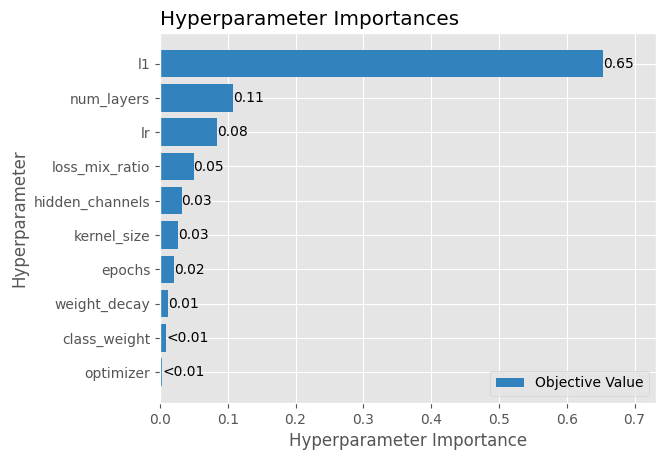
\includegraphics[width=0.8\textwidth]{figs/feature importance original.png}
    \caption{Hyperparameter Importance for the CNN Model with Original Features}
    \label{fig:hyperparams_importance_original}
\end{figure}

\begin{figure}[ht]
    \centering
    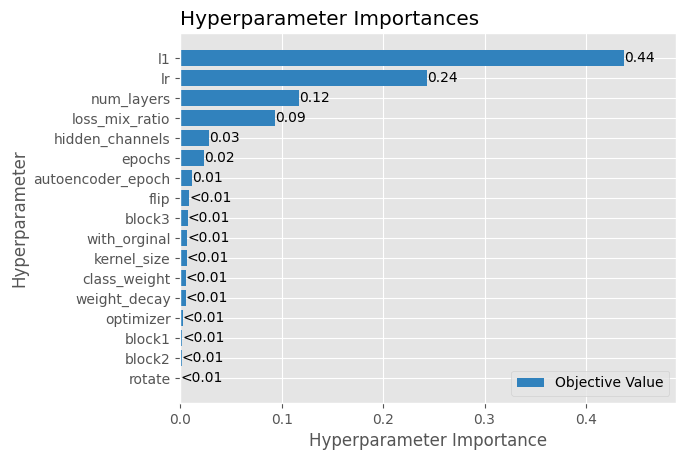
\includegraphics[width=0.8\textwidth]{figs/feature importance autoencoder.png}
    \caption{Hyperparameter Importance for the CNN Model with Autoencoder Features}
    \label{fig:hyperparams_importance_autoencoder}
\end{figure}

\subsection{Random Forest}
One of the main modeling approaches we focused on for this task is the random forest algorithm, applied to each pixel separately. This algorithm is an ensemble learning technique, meaning that it combines multiple smaller learners. During training, it builds multiple decision trees during training, with each trained on a random subset of the data (by bootstrapping) and using a random subset of features at each split. This is known as bagging or bootstrap aggregating. For prediction, it then aggregates (by mode) the predictions from the different trees to classify a point as a cloud or non-cloud. The goal is that this improves the model's robustness and ability to generalize as opposed to with a single learner. As RF is a general-purpose algorithm, the most significant assumption is that the spatial information is not important for the classification task as it is a pixel-wise classifier.

To enhance the performance of the random forest model, we conducted a search across various hyperparameters in the algorithm, including: the number of estimators, max depth of a tree, minimum samples in a split, minimum samples in a leaf, and the maximum number of features for a tree. Using Optuna, we efficiently searched through this hyperparameter space to find the optimal hyperparameters.

To get a robust sense of model performance, we used cross-validation. This was done by averaging the two sets of metrics generated by: training on labeled Image 0 and validating on labeled Image 1, and training on labeled Image 1 and validating on Image 0 (Image 2 was saved for the test set). After tuning the model through this hyperparameter search, the resulting metrics were: Macro F1: 0.7965 ± 0.0024, Accuracy: 0.7954 ± 0.0017, and ROC AUC: 0.9562 ± 0.0021 (these intervals were generated by averaging over 10 separate trials to account for the randomness in the process).


\subsection{Boosting}
Another algorithm we tested is XGBoost (which stands for Extreme Gradient Boosting), applied to each pixel separately. It is similar to the random forest in that it is an ensemble of decision trees, but different in that it applies boosting (gradient boosting) - it builds the ensemble sequentially, where each new tree corrects the errors of the previous ones. It optimizes performance using gradient descent. Overall, this method is also generalizable and robust as it is an ensemble method, and we can also compare the performance of boosting compared to bagging. Notice that it is a deterministic algorithm, so the standard deviation of its performance is 0. Similar to the random forest, the main assumption is that the spatial information is not important for the classification task.

Hyperparameter search for XGBoost involved a search space across number of estimators, maximum depth, learning rate, and regularization lambda. We again used Optuna to search through this space and find the optimal combination to maximize performance.

We again performed cross-validation over labeled Images 0 and 1 to get a sense of performance. After our hyperparameter search, our XGBoost performance metrics were: Macro F1: 0.8064, Accuracy: 0.8635, and ROC AUC: 0.9547. Despite the slightly higher metrics compared to Random Forest, we chose to focus our main predictions and analysis on the random forest model due to greater interpretability.


\subsection{Model Comparison}

Several insights emerge from the predictive modeling results, as shown in Table~\ref{tab:cv_performance}:

\begin{itemize}
    \item \textbf{Spatial information is critical for autoencoder features but not for original features.} RF and XGBoosting, which are pixel-wise classifiers, outperform the CNN on original features, while the CNN surpasses them on autoencoder or combined features. Notably, the selected CNN for original features uses a 1x1 kernel, acting as a pixel-wise classifier, reinforcing that spatial context offers little benefit for raw radiances. Conversely, the larger 7x7 kernel selected for autoencoder features highlights their reliance on spatial relationships, likely due to the autoencoder's reconstruction process spreading information across neighboring pixels. This explains why autoencoder features degrade RF and XGBoosting performance, as they cannot leverage spatial dependencies.

    \item \textbf{CNN with autoencoder features outperforms all models.} The CNN using autoencoder or combined features achieves the highest Macro F1 score and accuracy, surpassing other models in this study and the original paper's reported accuracy of 0.918 \cite{shi2008daytime}. This superior performance underscores the autoencoder's ability to extract robust, task-relevant representations for cloud detection.

    \item \textbf{Macro F1 provides a reliable lower bound on accuracy.} We selected Macro F1 as the primary metric to address significant variation in clouded pixel proportions across the three labeled images, ensuring balanced performance despite limited data. Cross-validation results confirm that accuracy never falls below Macro F1 by more than 0.01, offering a soft guarantee of robustness against distribution shifts in unseen images.

\end{itemize}

\subsection{Test Set Performance}

After selecting and tuning models using cross-validation on the training and validation images, we train the models with the full train/validation data and evaluate their performance on the held-out test image. Table \ref{tab:test_performance} summarizes the results for RF, XGBoost, and CNN models across different feature sets.

\begin{table}[ht]
    \centering
    \caption{Test Set Model Performance with Different Features.}
    \label{tab:test_performance}
    \begin{tabular}{cccc}
    \hline
    \textbf{Model}                 & \textbf{Features}                & \textbf{Macro F1 ± STD} & \textbf{Accuracy ± STD} \\ \hline
    \multirow{2}{*}{Random Forest} & Original Features Only           & 0.7711 ± 0.0049         & 0.7957 ± 0.0045         \\
                                   & Autoencoder or Combined          & 0.6969 ± 0.0022         & 0.7556 ± 0.0013         \\
    \multirow{2}{*}{XGBoost}       & Original Features Only           & 0.7198 ± 0.0000         & 0.7549 ± 0.0000         \\
                                   & Autoencoder or Combined          & 0.7073 ± 0.0000         & 0.7611 ± 0.0000         \\
    \multirow{2}{*}{CNN}           & Original Features Only           & 0.6054 ± 0.1191         & 0.6149 ± 0.1132         \\
                                   & Autoencoder or Combined          & 0.6937 ± 0.0565         & 0.6947 ± 0.0573         \\
    \hline
    \end{tabular}
\end{table}

The test set results reveal a significant drop in performance across all models and feature sets compared to cross-validation (Table \ref{tab:cv_performance}). The best-performing model from cross-validation, the CNN with autoencoder or combined features, achieves a Macro F1 score of 0.6937 and an accuracy of 0.6947 on the test set—far below its cross-validation scores of 0.9490 and 0.9581, respectively. Similarly, RF with original features, which scored 0.8557 (Macro F1) and 0.8542 (accuracy) in cross-validation, drops to 0.7711 and 0.7957. XGBoost and other configurations exhibit comparable declines. Even more striking are the high standard deviations for CNN models (e.g., 0.1191 for Macro F1 with original features), indicating instability across test predictions.

This consistent underperformance suggests a distribution shift between the training/validation images and the test image. Given only three labeled images—two for training/validation and one for testing—variations in cloud patterns, radiance distributions, or spatial characteristics likely differ significantly across images. The CNN with autoencoder features, despite its superior cross-validation performance, appears particularly sensitive to this shift, possibly due to overfitting to spatial patterns in the training data that do not generalize.

All models now perform poorly relative to expectations set by cross-validation and the original paper's benchmark of 0.918 accuracy \cite{shi2008daytime}. This degradation highlights the limitations of training on such a small labeled dataset, where capturing the full variability of MISR images is infeasible. While the autoencoder aimed to enhance feature robustness, its benefits diminish under distribution shift, and pixel-wise models like RF and XGBoost fare only marginally better. Further exploration to confirm and mitigate this shift—such as analyzing feature distributions across images-requires additional labeled data, which is beyond the scope of this lab.

The remaining sections will focus on post-hoc analysis, feature importance, and stability analysis instead of predictive modeling, to reveal insights into model behavior and potential improvements for future work.

% Develop several (i.e., at least three) 0-1 classifiers for the presence of clouds, using your best features and autoencoder features, or others, as necessary. Provide a brief description of the classifier, state the assumptions of the classification models if any, and test if the model assumptions are reasonable.

% RF, SVM, XGBoost, etc. I'll also do a lightweight CNN model.

% Assumption: RF, SVM, and XGBoost assume the label is solely determined by the pixel's features. CNN assumes the label is determined by the pixel's features and its neighbors.

% Try the original features, the autoencoder features, and the combination of both.

% Assess the fit for different classification models e.g. using cross-validation, AIC, and/or the ROC curve. Think carefully about how to choose folds in cross-validation and/or your training/test splits.

% Justify our choice of evaluation metrics (Marco F1 score and accuracy). This choice stems from the fact that the proportion of clouded pixels differs significantly between images, and we only have three images. The Marco F1 score (used for model selection) leans towards the robustness of the model, ensuring that the model does not degrade too much when the distribution shifts. Accuracy is the aimed metric for the task. Use the Marco F1 score instead of the micro F1 score because we want to make it symmetric between the two classes as we have no preference for either class.

% The scheme of the CV should already be justified in the EDA section.

% Also, include a simple thresholding model as a baseline. (As in the original paper)

\section{Feature Importance Analysis Based on the RF Classifier}
To gain more interpretability for our modeling approach, we conducted extensive feature importance analysis for the Random Forest model. Before including the autoencoder, we can understand original feature importances from a model that uses only the original 8 features from the labeled images. We analyze this using scikit-learn's built-in functionality for importances, which measures feature importance as a mean decrease in impurity. 

\begin{figure}[ht]
    \centering
    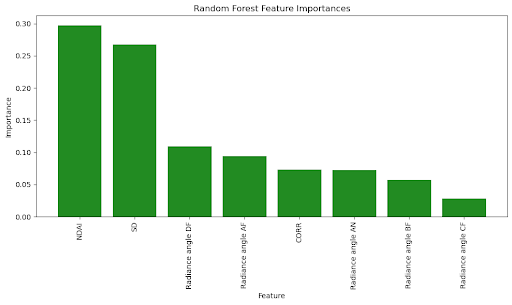
\includegraphics[width=0.5\textwidth]{figs/orig_features_only_feature_importances.png}
    \caption{Feature Importances for Random Forest Model with Original Features}
    \label{fig:orig_features}
\end{figure}

The results are shown in Figure \ref{fig:orig_features}. From this model, we can see that the random forest algorithm emphasizes the NDAI and SD features by a significant margin, followed by all of the radiance angles.

We again repeat a similar analysis but with the full model utilizing both original and autoencoder features. One approach is to restrict our visualization to solely the original features, so that we can see their importance relative to each other in the presence of autoencoder features. 

\begin{figure}[ht]
    \centering
    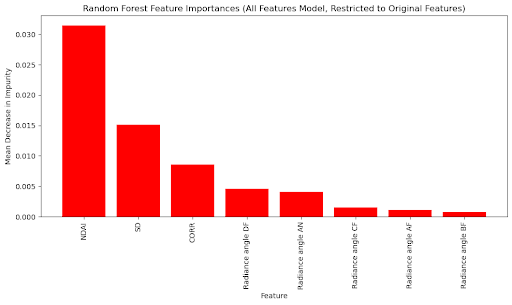
\includegraphics[width=0.5\textwidth]{figs/full_model_restricted_feature_importances.png}
    \caption{Feature Importances for Full Random Forest Model [only showing original features]}
    \label{fig:restricted_feature_importances}
\end{figure}

As shown in Figure \ref{fig:restricted_feature_importances}, it reveals the interesting takeaway that CORR now becomes more important than all of the radiance angles, whereas before adding autoencoder features, it had less importance than some radiance angles. Perhaps this suggests that autoencoder features subsume some of the information of radiance angles.

Finally, we can view the feature importances with no restrictions, for all features. This allows us to understand the relative importance of original features vs. autoencoder features.

\begin{figure}[ht]
    \centering
    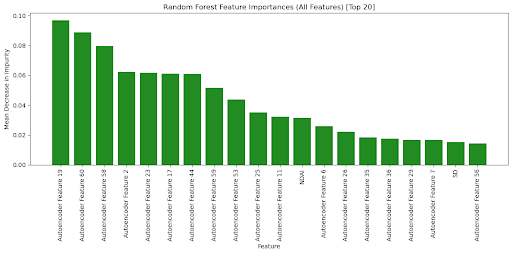
\includegraphics[width=0.5\linewidth]{figs/full_model_all_feature_importances.png}
    \caption{Features Importances for Full Random Forest Model [all features, top 20 displayed]}
    \label{fig:all_feature_importances}
\end{figure}

From Figure \ref{fig:all_feature_importances}, we can see that the majority of the 20 most important are from autoencoder features, meaning that the full model has shifted toward emphasizing the autoencoder features more. However, NDAI and SD also appear in the top 20, suggesting that they are still leveraged and not fully overshadowed.

\section{Post-hoc Analysis}

% Pick a good classifier. Show some diagnostic plots or information related to convergence, parameter estimation (depending on your choice of models), and feature importance. The last item will be especially interesting after all of our effort spent engineering good features. Some examples of useful techniques are MDI+, coefficient magnitudes, permutation importance, etc.

% I recommend using the RF or XGBoost model for this part as you are more familiar with them. The feature importance can have two perspectives: (1) See the autoencoder features as a black box and see how much they contribute to the prediction, compared to the original features. (If your model uses both of them) (2) See the importance of the original features. Permute the original features before sending them to the autoencoder to avoid the "black box".

% For your best classification model(s), perform some post-hoc EDA. Do you notice any patterns in the misclassification errors? Again, use quantitative and visual methods of analysis. Do you notice problems in particular regions or specific ranges of feature values?

% I don't have a specific recommendation for this part. You can try to visualize the feature importance, the confusion matrix, or the ROC curve. You can also try to visualize the misclassified pixels.

% How well do you think your model will work on future data without expert labels? Is there a stability analysis, or some test that might give you a good idea of this? Investigate how your results change when you conduct various perturbations throughout your prediction pipeline. As a sanity check, run your classifier on some of the unlabeled images to see if the predictions look reasonable.

% Stability: Can be just bootstrapping the data and see how the model changes. Can only do it for 1 model. Add noise to the data and see how the model changes if you want to be more thorough but I don't like this idea.

% Are there any other perturbations that are reasonable? I see few judgment calls we made in the pipeline that could be perturbed.

% Sanity check: Run the model on the unlabeled images and see if the prediction makes sense. I'm not sure how to distinguish clouded pixels from non-clouded pixels in the unlabeled images by eye though but you can try.

% Test set: Run our models on the test set and report the accuracy, Marco F1 score, and ROC if you think it's necessary. Claim if the test performance is reasonable good or not.

To understand our prediction performance in more depth, we conducted extensive post-hoc EDA. We can visualize our predictions compared to the true cloud/non-cloud pixels in the test image to have a better sense of the model's patterns in prediction. The results are shown in Figure \ref{fig:prediction_plot}.

\begin{figure}[ht]
    \centering
    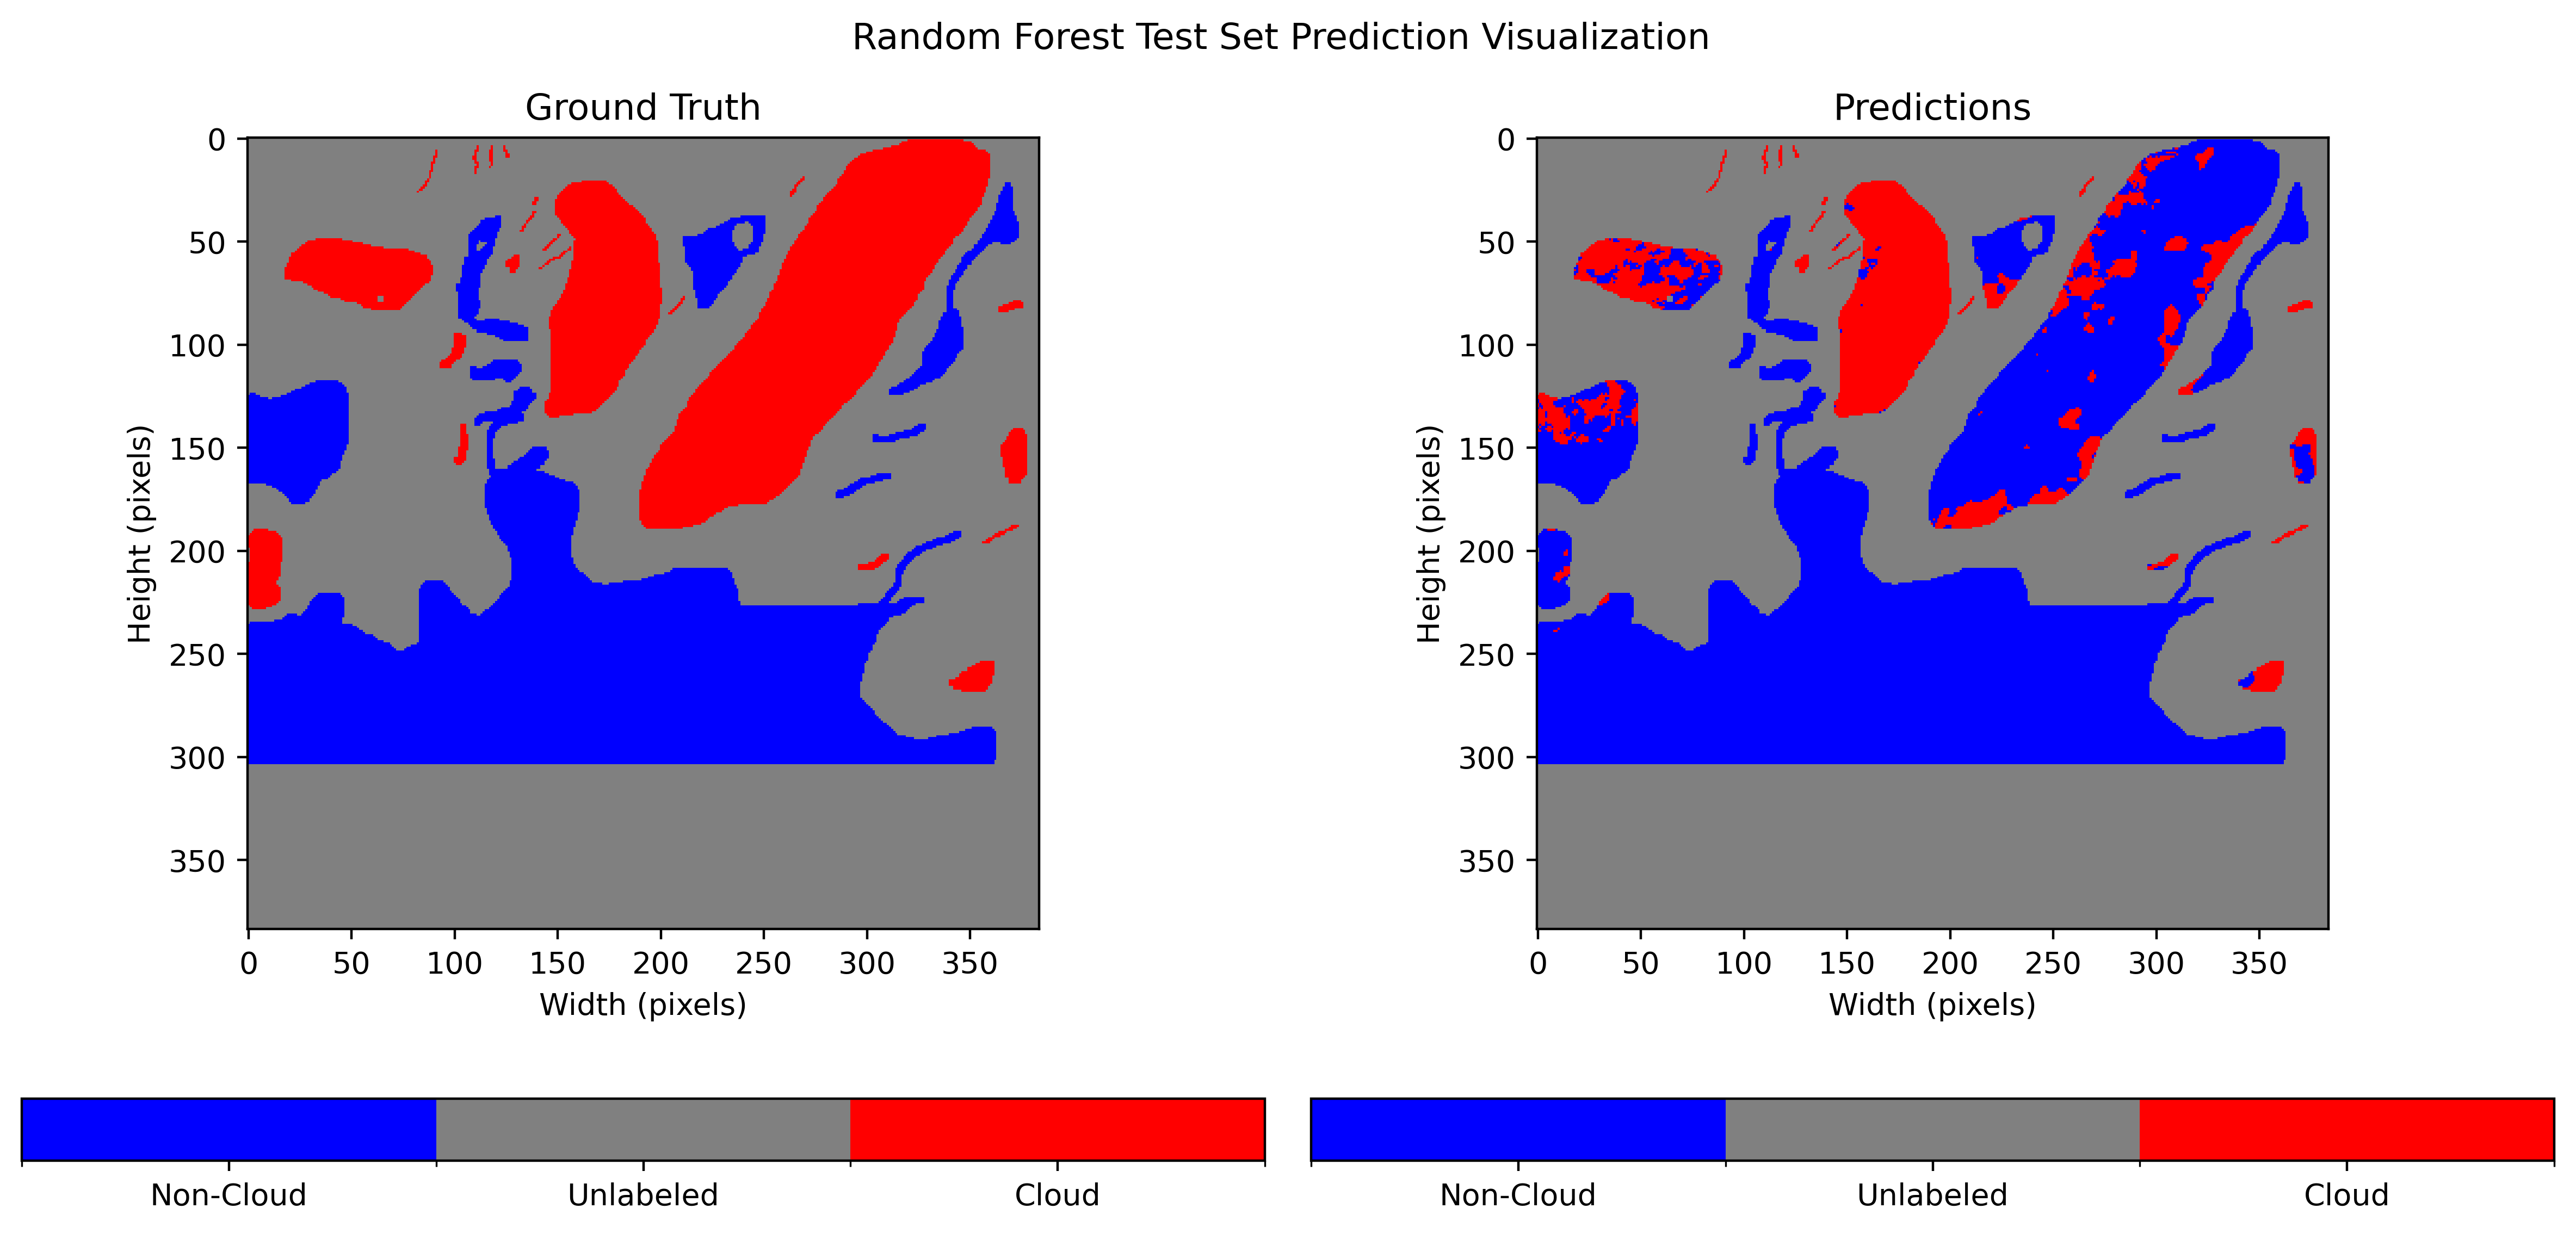
\includegraphics[width=0.75\linewidth]{figs/pred_plot.png}
    \caption{Image Prediction: Ground Truth vs Random Forest}
    \label{fig:prediction_plot}
\end{figure}

Looking at the visualized prediction comparison, we can see many patterns in the errors. We see that the majority of errors are predicted non-cloud (blue) areas that should be cloud (red) areas. This highlights that the model has better relative precision than recall since it often misses some true cloud (red) areas. This is why we prioritize Macro F1 throughout these experiments to try to balance these metrics. Visually, we can notice that the bulk of misclassifications are concentrated in the large true cloud mass at the top right section of the image, with many adjacent pixels being wrongly labeled as non-cloud. This is interesting as this area makes up the vast majority of errors and is closely concentrated. One anomaly in the other direction, i.e. true non-clouds that were mistakenly predicted as clouds, is concentrated in the middle-left area.

To understand this from a more quantitative standpoint, we conducted further error analysis. We utilized spatial autocorrelation analysis to understand in a quantitative sense how concentrated errors are, whether they were more scattered or close to each other. This method of autocorrelation measures how similar the error map is to a shifted version of itself. As shown in \ref{fig:spatial_error_correlation}, high values in the center of this plot indicate that errors are strongly correlated with themselves. This means that errors appear in groups/clusters, which aligns with intuition from glancing at the prediction plot. This is in contrast to if the high values were away from the center, which would indicate a correlation of errors with errors at a distance, meaning more scattered errors.

\begin{figure}[ht]
    \centering
    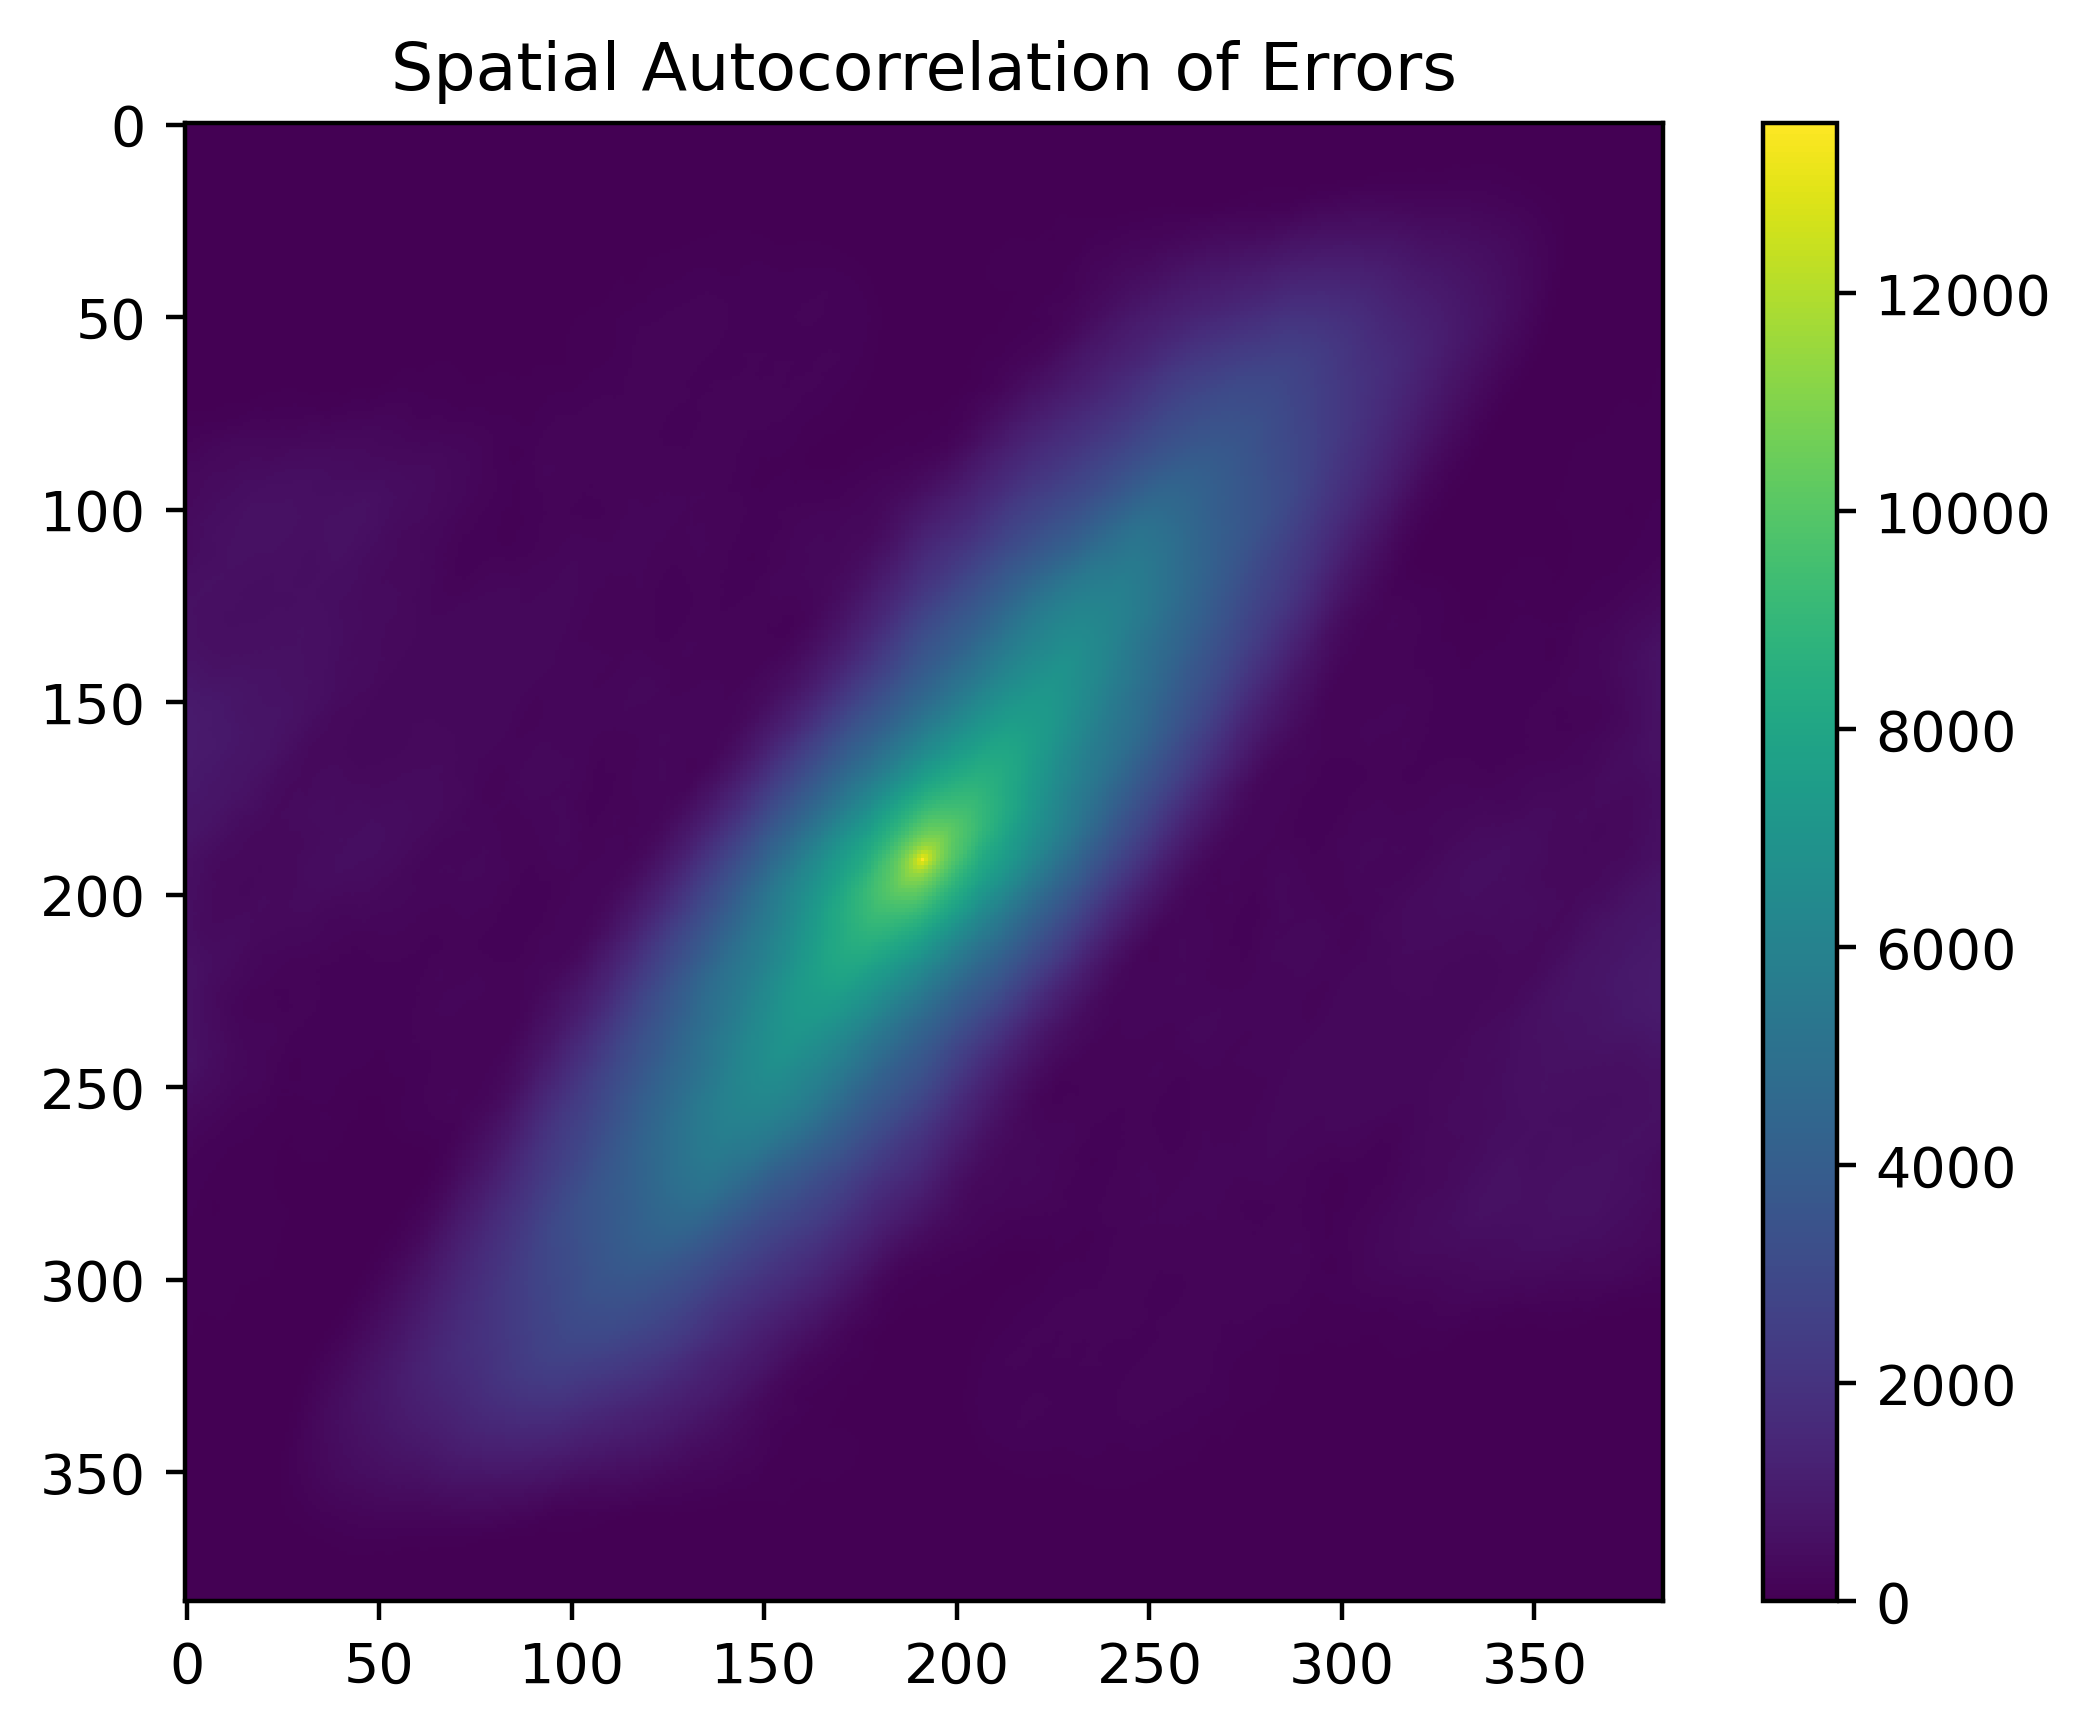
\includegraphics[width=0.5\linewidth]{figs/spatial_error_correlation.png}
    \caption{Spatial Autocorrelation of Errors for Random Forest Model Prediction}
    \label{fig:spatial_error_correlation}
\end{figure}

Lastly, we investigated feature values to search for patterns in the misclassifications. For each of the original features (since they are more interpretable than the autoencoder features), we compared the distribution of the feature in the correctly classified regions to the incorrectly classified regions, to look for any distributional shift patterns of certain features occurring with misclassifications. The majority of them do not show signs of major distributional shifts, meaning that the misclassifications are likely not skewed because of one specific feature but rather a combination. Most of these images have been excluded for brevity, but one highlighted in \ref{fig:radiance_angle_an_dist_comparison} is for radiance angle AN, which seems to contain the largest distributional shift between the misclassified and correct groups. This reveals the pattern that the misclassified group seems to have a slightly higher-valued concentration of radiance angle AN.

\begin{figure}[ht]
    \centering
    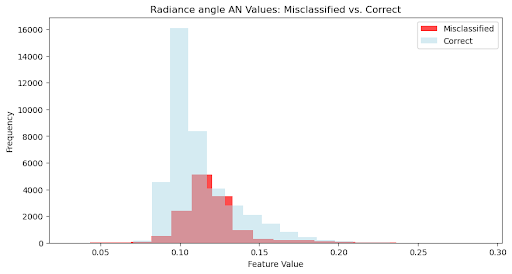
\includegraphics[width=0.5\linewidth]{figs/radiance_angle_AN_dist_comparison.png}
    \caption{Feature Distribution Comparison of Misclassified and Correct Predictions: Radiance Angle AN}
    \label{fig:radiance_angle_an_dist_comparison}
\end{figure}

\section{Stability Analysis}
We conducted stability analysis to get a better sense of how the model might work on future data, as well as a general sense of the robustness of our model. One approach to this was making a perturbation on the features so that we could examine how sensitive our model is to changes in features. To make a more realistic perturbation compared to random noise, we used a Gaussian filter to apply a smoothing/blur over features, before adding a small amount of Gaussian noise. We claim that a Gaussian filter and noise is a reasonable perturbation because it mimics a real-world scenario where the features might be slightly blurred or noisy, or denoised algorithms might be applied to the features. We then conducted this over several separate trials and analyzed how many of the resulting predictions (including the original) agreed with each other, creating a disagreement map as shown in Figure \ref{fig:feature_gaussian_filter_disagreement}. A value of 0 indicates full agreement, while a value of 1 indicates disagreement. As shown, our model seems quite robust, as the majority of the predictions remain in agreement after these perturbations over 10 separate trials. This was tested over various values of sigma (the standard deviation of the Gaussian filter), one of which is shown and shows good stability despite a standard deviation of 2 [other values omitted for clarity]. Overall, we can conclude from this experiment that the model is relatively stable and robust to these semi-realistic feature perturbations.

\begin{figure}[ht]
    \centering
    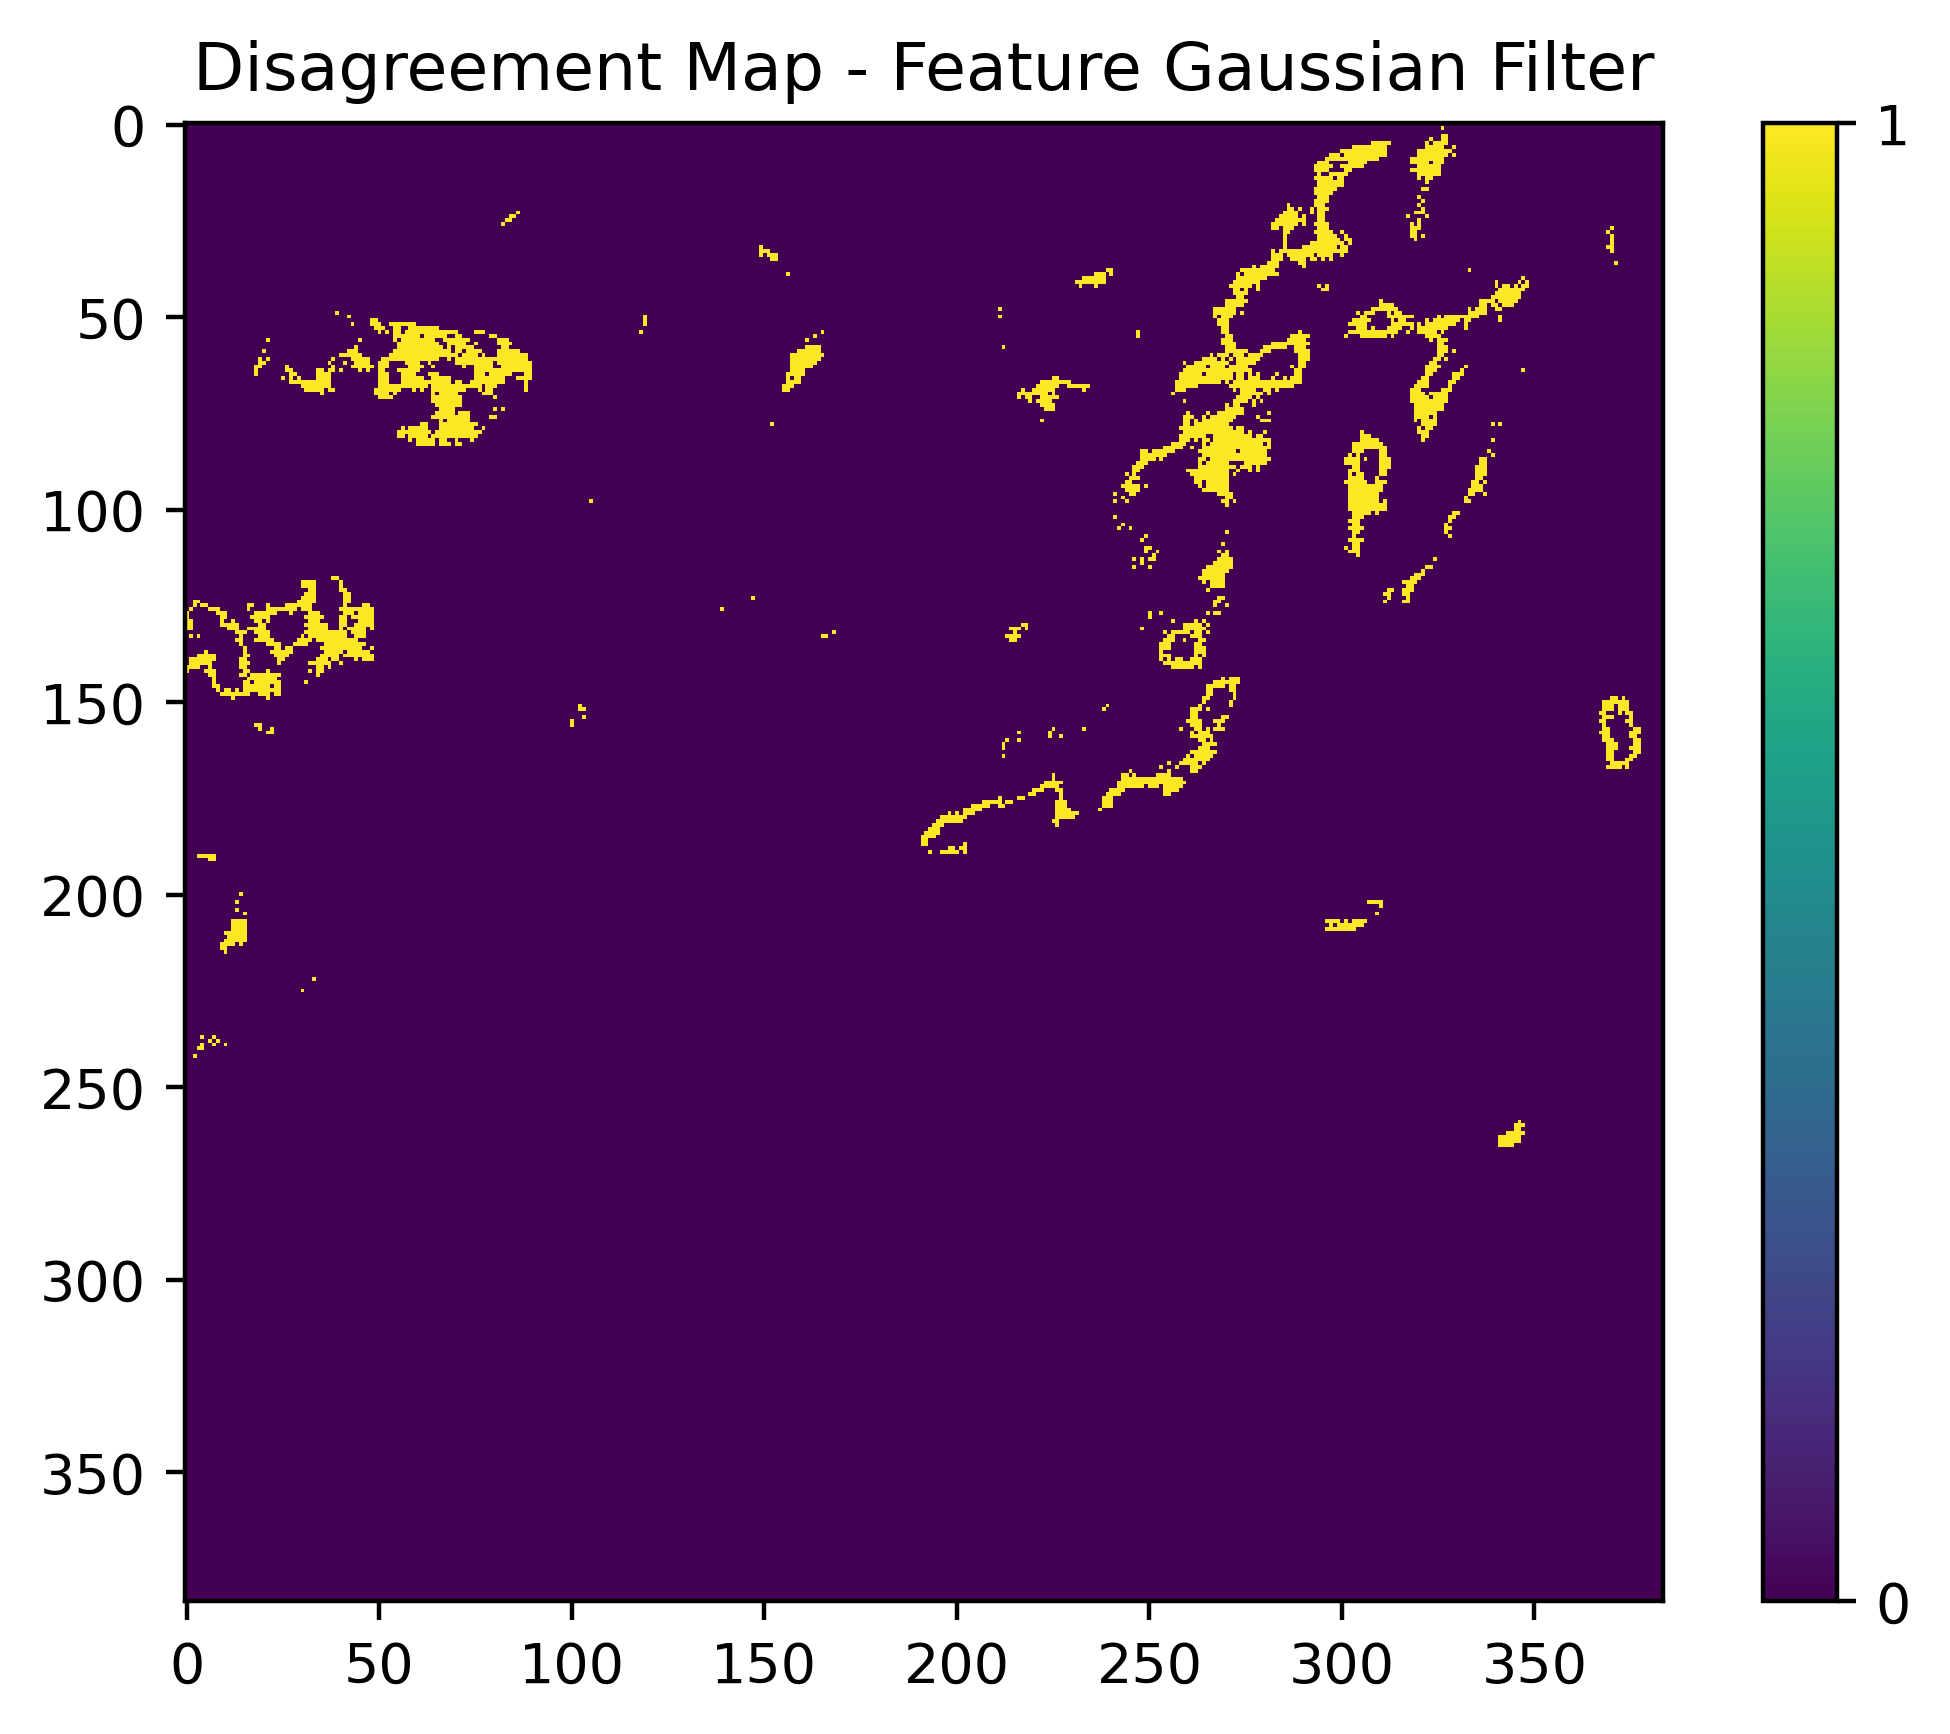
\includegraphics[width=0.5\textwidth]{figs/feature_gaussian_filter_disagreement_map.png}
    \caption{Prediction Disagreement after Feature Gaussian Filter Perturbation}
    \label{fig:feature_gaussian_filter_disagreement}
\end{figure}


To understand how perturbations at various stages of the prediction pipeline affect the model, we also analyzed the effect of perturbations at the post-processing stage by applying Gaussian smoothing to our predictions. This helps get a sense of the uncertainty/confidence of the model (i.e. making “clearer” predictions rather than borderline ones that switch between cloud vs. non-cloud if slightly perturbed). For the example of a standard deviation of 0.5 used for the smoothing, we can see that some predictions start to change, though the majority remain relatively stable as shown in Figure \ref{fig:post_processing_perturbation}. However, for larger values of the Gaussian filter standard deviation, we see more labels flip. This suggests that the next step could be aiming to reduce model uncertainty and make the model more stable for these types of perturbations.

As a sanity check, we also confirmed that our model's predictions on unlabeled images look reasonable and align with domain knowledge from the paper, suggesting that our model matches what we expect in reality.

\begin{figure}[ht]
    \centering
    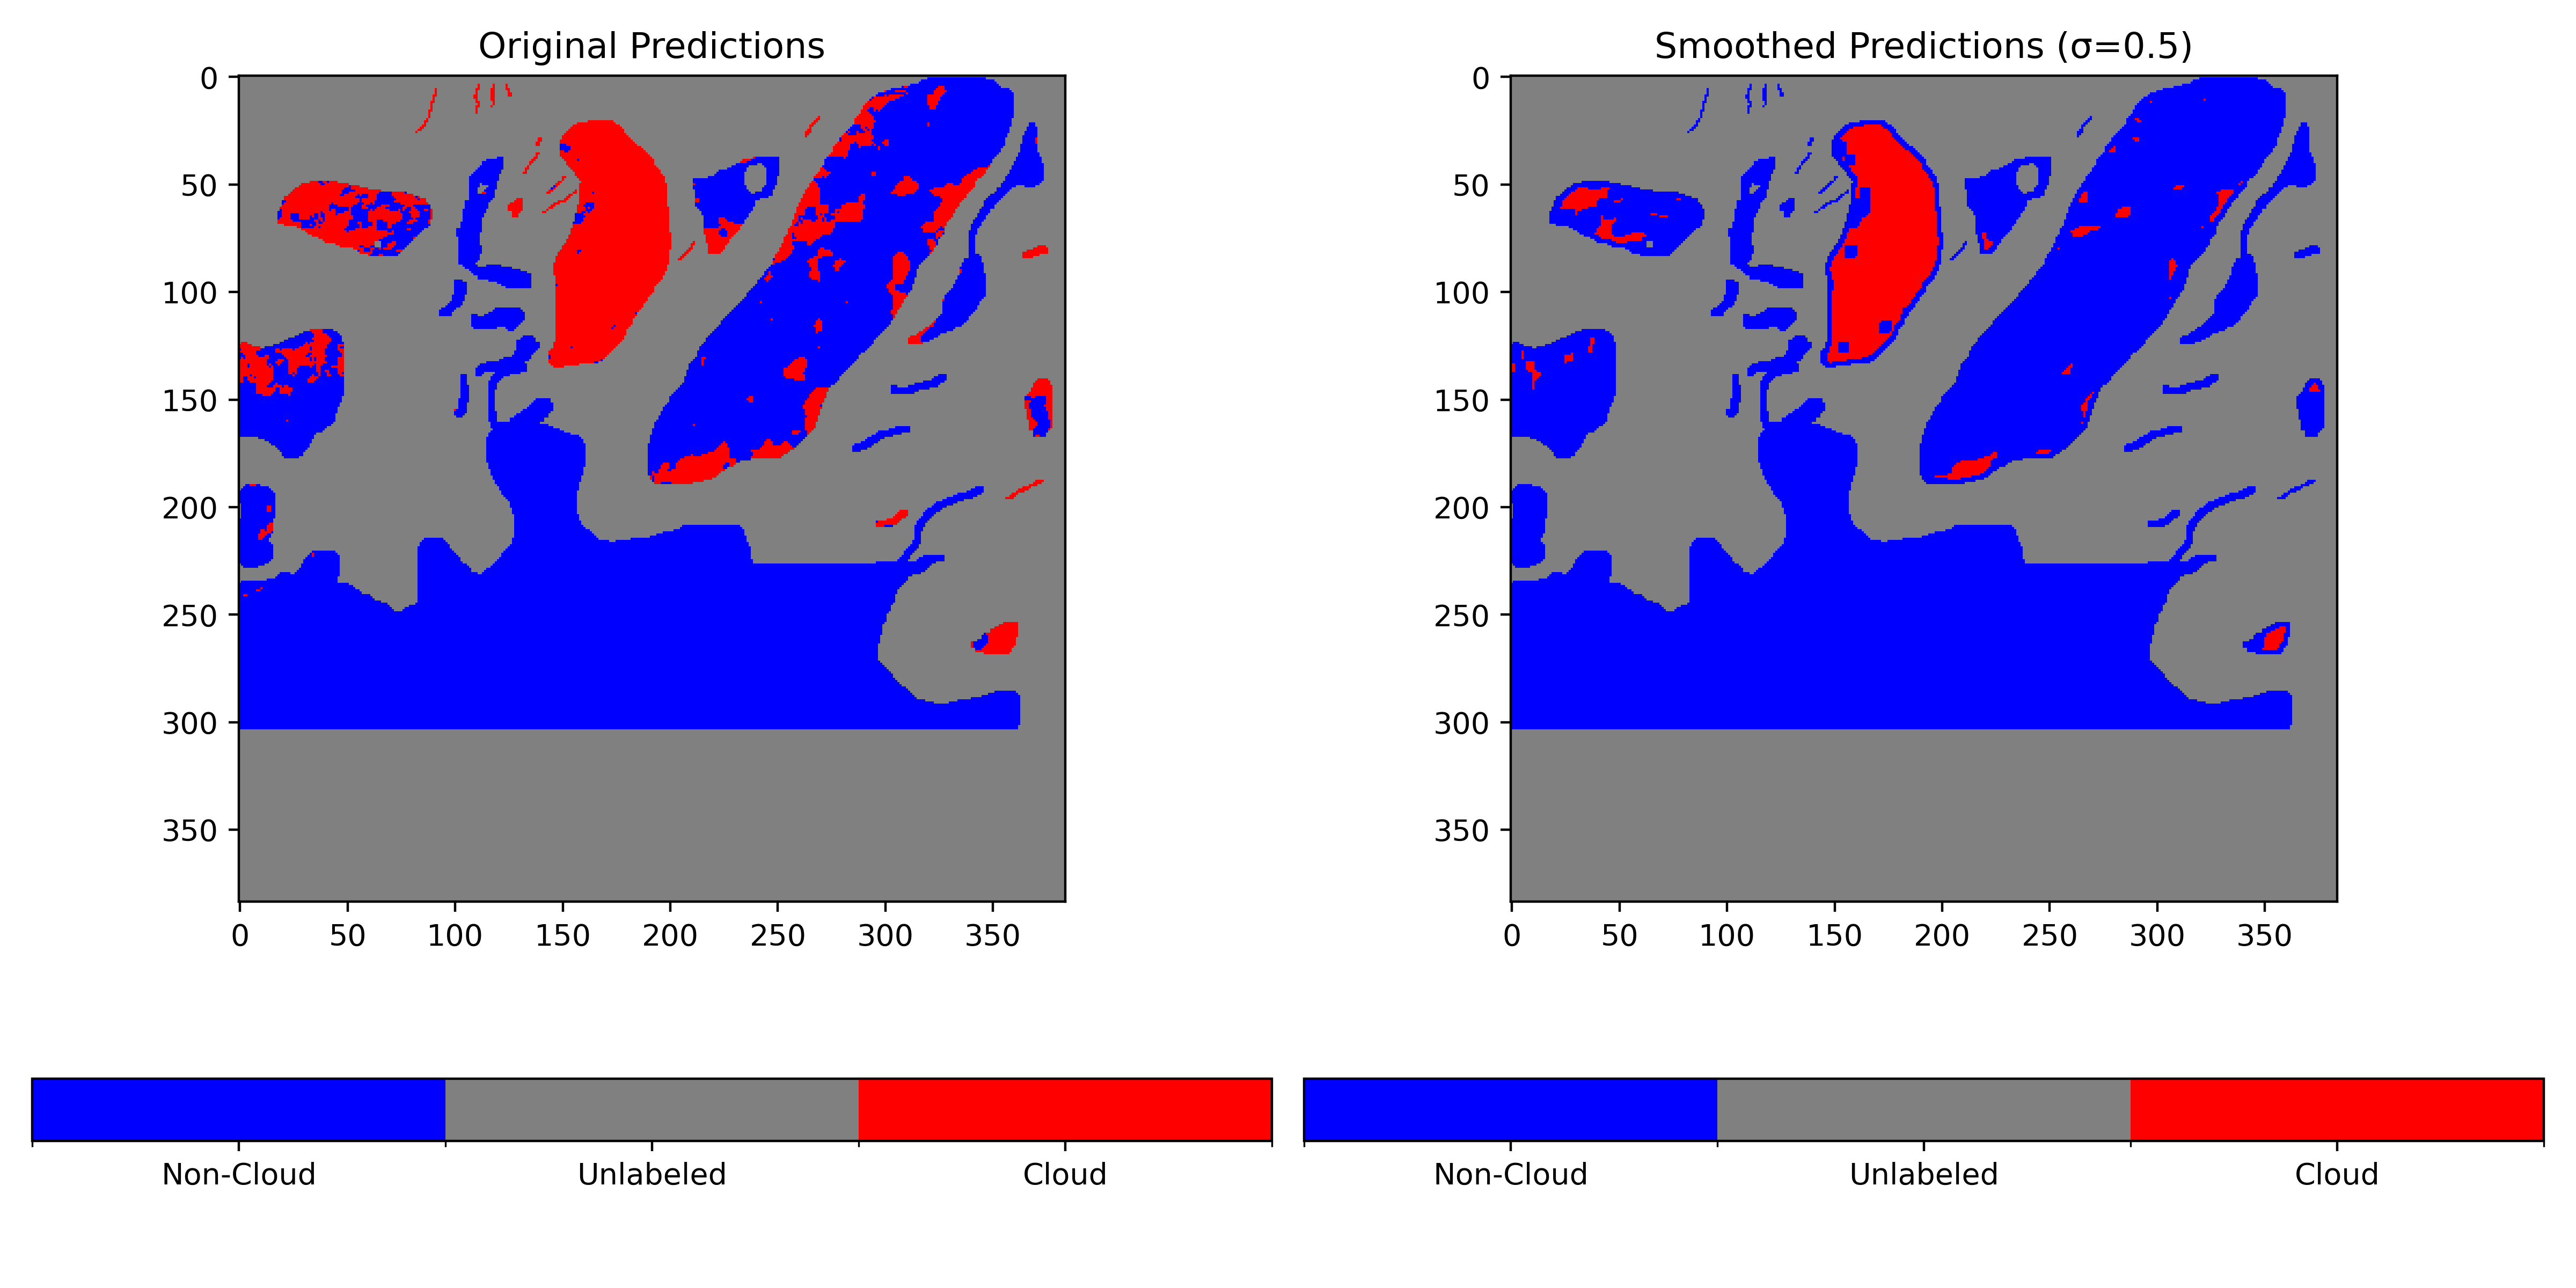
\includegraphics[width=0.75\linewidth]{figs/post_processing_perturbation.png}
    \caption{Post-Processing Gaussian Smoothing Perturbation Prediction Comparison}
    \label{fig:post_processing_perturbation}
\end{figure}

\section{Conclusion}

In this lab, we explored the full pipeline of cloud detection in MISR images, from feature engineering to predictive modeling and post-hoc analysis. We began by extracting original features and autoencoder features, then trained several classifiers, including Random Forest, XGBoost, and a lightweight CNN, to predict cloud presence. Our results showed that the CNN with autoencoder features outperformed other models in the cross-validation setting. However, the test set performance revealed a significant drop in accuracy and Macro F1 scores, indicating a distribution shift between the training/validation images and the test image. Post-hoc analysis provided insights into the model's prediction patterns, feature importance, and stability. Our feature importance analysis highlighted the importance of the derived autoencoder features, while the stability analysis demonstrated the model's robustness to feature perturbations. Future work could focus on improving model generalization and stability, potentially through more extensive data augmentation or regularization techniques.

\newpage

\printbibliography

\appendix
\section{Academic honesty}
\subsection{Statement}
We affirm that the work in this report is entirely my own. We have not copied from any unauthorized sources, and all contributions from classmates, external sources, or tools are acknowledged. Academic research honesty is necessary because it ensures fairness, builds trust in scholarly work, and reflects personal integrity. Misrepresenting work not only undermines academic standards but also disrespects the time and effort of peers and educators. Maintaining honesty in research fosters a learning environment where collaboration and progress can thrive authentically.

\subsection{LLM Usage}

We used ChatGPT to assist in clarifying concepts, creating visualizations, checking grammar, and improving the structure of our explanations. No content of the report or code was generated by the LLM without our review, editing, and refinement. We ensured that all content was written and understood by us, and the LLM was used as a tool to enhance our work rather than replace our understanding, we take full responsibility for all content in the report.

\end{document}